%implementing document formatting:
\input{preambleNy.tex}
\input{macros.tex}
\begin{document}

%||||||||||||||||||||||||||||||||||||||||||||||||||||||||||||||||
%|||||||				Example Inputs					 ||||||||
%||||||||||||||||||||||||||||||||||||||||||||||||||||||||||||||||
%|||||||												 ||||||||
%	\input{rapportAfsnit/zExamples/aFigureSample.tex}	%||||||||
%	\input{rapportAfsnit/zExamples/bTableSample.tex}	%||||||||
%	\input{rapportAfsnit/zExamples/cEquationSample.tex}	%||||||||
%|||||||												 ||||||||
%||||||||||||||||||||||||||||||||||||||||||||||||||||||||||||||||
%||||||||||||||||||||||||||||||||||||||||||||||||||||||||||||||||
%\iffalse
%--------------------Introduktion--------------------------------
\chapter{Indledning}\label{Indledning}
% !TeX spellcheck = da_DK
\subsection{Indledning}
heuhkehhorho
\input{rapportAfsnit/bInitierende/initierende_spg}

%-----------------------Problemanalyse---------------------------
\chapter{Problemanalyse}
% !TeX spellcheck = da_DK
\subsection{Amyotrofisk Lateral Sklerose}
.....skriv noget her...
%\subsection{Følger}

ALS er en individuel sygdom og sygdommens forløb vil ligeledes variere fra patient til patient. Dog kan der være fællestræk for sygdommens progression, men med undtagelse af nogle patienter. Man kan inddele sygdommen i 3 stadier, et tidligt stadie, et mellem stadie og et sent stadie. I de tidligste stadier er der mulighed for, at patienterne kan ignorere symptomerne og diagnosticeres oftest efter dette stadie. [1] Disse symptomer kan være milde og kun påvirke mindre dele af kroppen, hvor musklerne eksempelvis kan være svage eller stive. Dette vil ligeledes have påvirkning på patientens balance. I det midterste stadie vil symptomerne begynde at udbrede sig. Nogle muskler kan være paralyserede, hvor andre eksempelvis kan være upåvirkede. Andre muskler vil blive svagere med tiden og dette vil blandt andet medføre problemer med synkning og vejrtrækningen. I de senere stadier vil de fleste voluntære muskler vil være paralyserede og det vil måske ikke være muligt at indtage føde eller væske. Herudover vil det for oftest i dette stadie ikke være muligt at trække vejret grundet respirationssvigt. [1] 

Symptomerne behøver nødvendigvis ikke at ramme begge ben samtidig. Til at starte med at mindre symptomer som besvær ved at gå op ad trapper. Ligeledes kan det være patienterne vil begynde at være nødsaget til at trække benet for at kunne gå. Herefter vil det musklerne gradvist blive svagere og med tiden vil de ikke længere være i stand til at gå. [2]



1: https://www.mda.org/disease/amyotrophic-lateral-sclerosis/signs-and-symptoms/stages-of-als 
2: http://patient.info/health/motor-neurone-disease-leaflet 
 Denne skal ikke være med i master dokumentet. 
\subsection{Livskvalitet hos ALS-patienter}
% mere konkret omkring deres livskvalitet og familieforhold
% tilføj tabel 2 fra ilse2015
Livskvaliteten hos patienter med ALS undersøges for at vurdere, hvilken påvirkning sygdommen samt dens progression har på patienten. Der er ingen behandling for at stoppe sygdomsprogressionen, men der eksisterer forskellige palliatative behandlinger \citep{neudert2004}. Det er fordelagtigt at kende patienternes livskvalitet for at vurdere den optimale palliative behandling \citep{ilse2015}.

Livskvalitet defineres ud fra en persons fysiske sundhed, psykologiske tilstand, grad af selvstændighed, sociale relationer og personlig tro \citep{pagnini2013}.

Der kan fremhæves to forskellige typer af livskvalitetsvurderinger: en overordnet livskvalitet og en sundhedshedsrelateret livskvalitet. 
Den overordnede livskvalitet relaterer til patienternes samlede livskvalitet, og den sundhedsrelaterede livskvalitet dækker over de fysiologiske og mentale aspekter ved sygdommen \citep{ilse2015, nuedert2004}. Da ALS påvirker patienters fysiske formåen, ses der et fald i denne type livskvalitet, som sygdommen fremskrider \citep{ilse2015}. Dette fremgår ligeledes af \autoref{tab:livskvalitet}, der viser en forringet livskvalitet hos ALS-patienter når der sammenlignes med resten af befolkningen. Livskvaliteten vurderes ud fra mobilitet, selvpleje, udførelse af normale aktiviteter, oplevelse af smerte eller ubehag samt diagnoser som angst og depression, hvor næsten 3 gange så mange ALS-patienter lever med disse problemer sammenlignet med den resterende befolkning.

\begin{table}[H]
\centering
\begin{tabular}{l| l| l}
\multicolumn{3}{c}{\textbf{Moderate eller alvorlige problemer målt ud fra europæisk livskvalitetsvurdering}}
   \\
                                                                         & ALS-patienter                                    & Normativ tysk population                                   \\
                                                                         \hline
                                                                  
Mobilitet                                                                & 83,7 \%                                          & 16,6 \%                                                    \\
Selvpleje                                                                & 77, 6 \%                                         & 2,9 \%                                                     \\
Normale aktiviteter                                                      & 85,7 \%                                          & 10,2 \%                                                    \\
Smerte eller ubehag                                                      & 61,2 \%                                          & 27,9 \%                                                    \\
Angst eller depression                                                   & 67,4 \%                                          & 4,4 \%                                                    \\
\end{tabular}
\caption{Tabellen sammenligner livskvaliteten for ALS-patienter med livskvaliteten for den tyske population. Det ses heraf at ALS-patienter har en forringet livskvalitet i forhold til den resterende tyske befolkning.\citep{ilse2015} (Revideret)}
\label{tab:livskvalitet}
\end{table}

\noindent
Til trods for, at der sker et fald i den sundhedsrelaterede livskvalitet, er der tidligere vist, at den overordnede livskvalitet forbliver stabil \citep{ilse2015, nuebert2004}. Dette kan forklares ved et "response shift" eller "frame shift", der er en måde at håndtere sin sygdom, hvor social støtte under sygdomsforløbet vægtes højere end normalt i bestemmelsen af livskvalitet \citep{ilse2015}. Af denne grund foreslås det, at faldet i sundhedsrelateret livskvalitet i forhold til mobilitet og selvhjælp afhjælpes ved teknologiske hjælpemidler. På denne måde vil ALS-patienternes sociale interaktioner kunne have fokus på deres sociale netværk, da disse sociale interaktioner er begrænsede på baggrund af ALS \citep{ilse2015,tramonti2012}.







% Jeg ved ikke, om dette er nok. Men jeg tænker, at vinklingen er mere som den, vi snakkede om. Der kan sandsynligvis sagtens tilføjes noget hertil - evt. tænker jeg, om man vil kunne tilføje (noget af?) tabel 2 fra ilse2015 for at få nogle tal på bordet. 
% Mads: Det er min hensigt at lave en form for afgrænsning til de fysiske mangler ved at tage udgangspunkt i den sundhedsrelateret livskvalitet og det med at den forringes i takt med at de oplever større svaghed i musklerne. 
%Tænker det er en afgrænsning vi bliver nød til at fortages os, for jeg synes ikke at kunne finde litteratur der giver den nødvendige relation mellem det at jeg skal fokusere på besværligheden i at gå.
% !TeX spellcheck = da_DK
\section{Teknologier og hjælpemidler til brug ved ALS} \label{sec:teknologier}
Som tidligere nævnt er ALS en livstruende sygdom, hvor følgerne udvikler sig gradvist, hvilket gør, at patienternes funktionelle evner svækkes over sigt, hvorfor der er behov for en række hjælpemidler, som helt eller delvist kan være en hjælp i hverdagen. Nogle af hjælpemidlerne anvendes i starten af sygdommen, således patienterne kan klare sig selvstændigt, hvor der senere er behov for andre hjælpemidler samt helt eller delvist hjælp fra familie eller plejepersonale. \citep{brandt2010}

\subsection{Teknologiske og personlige hjælpemidler}
De mest anvendte hjælpemidler for ALS-patienter kan være kørestole, toiletstole og stokke. Hjælpemidlerne er alle redskaber, der støtter og aflaster patienten. Derudover kan der anvendes mere individuelt tilpassede hjælpemidler til hver enkelt patient. Dette kan f.eks. være tilpassede kørestole, fodtøj eller høreapparater. \citep{brandt2010}

Der er, som tidligere nævnt, mange patienter, der oplever respirationproblemer sent i sygdomsforløbet, hvorfor respirationshjælp er nødvendigt \citep{hefferman2006}. Der kan anvendes medicin som antibiotika, lindrende behandling og/eller hjælpemidler som forskellige respiratorer til at lindre og håndtere vejrtrækningsproblemerne. Ved brug af respirator, bliver patienterne i højere grad afhængige af hjælp, da det kræver plejepersonale at betjene denne. \citep{rcfm2001}

\subsubsection{Udfordringer ved brug af hjælpemidler}
%overskrift
Som nævnt i \autoref{sec:teknologier} mister patienter muskelkraft, som sygdommen udvikler sig, og de bliver derfor mere og mere afhængige af hjælpemidler, da tabet af muskelkraft til sidst medfører, at kørestolsbrug kan blive nødvendigt. På denne måde forsvinder patienternes selvstændighed, da de er afhængige af hjælpemidler samt assistance fra plejepersonale eller familie. \citep{brandt2010} Dette fører til nogle begrænsninger for patienten og medvirker til en forringet livskvalitet. En mulig måde at give ALS-patienter nye muligheder er anvendelse af et body augmentation-system, hvilket bidrager som et supplement af tabte kropsfunktioner. \citep{erlen2003} 

\subsection{Body augmentation som hjælpemiddel}
Én form for body augmentation er et exoskelet. Et exoskelet  anvender biologiske signaler, og kombinerer disse med kraften fra en maskine. På denne måde er det muligt, at maskinen fungerer som en menneskelig operatør, som kan forbedre menneskets styrke eller genoprette bevægelse. \citep{yang2008} Dette gør, at exoskelettet kan anvendes som et hjælpemiddel til patienter, som lider af handicap eller skader, hvorved exoskelettet gør det muligt at aflaste patienten. \citep{bogue2015} 

Forsøg har påvist, at det er muligt for patienter, som er lammet fra brystet og ned, at gå ved brug af exoskelet for patienter. Exoskelettet kan registrere, når patienten bevæger sig til siden og herved hjælpes benene til at gå, selvom patienten er uden muskelkraft og følesans. Foruden fordele ved at gå, formodes det, at det har en positiv indflydelse på patientens kredsløb, knogler, led og fordøjelse. \citep{regmidt2015} 
% !TeX spellcheck = da_DK
\section{Gangfunktion}
Efterhånden som ALS-patienter mister muskelkraft, vil bevægeligheden i deres led nedsættes. Af denne grund opstår der kontrakturer i led, og muskelstramninger i de omkringliggende muskler.

Ved gang anvendes knæ-, hofte- og ankelleddet, hvilket fremgår af \autoref{fig:knaet}, hvis disse led ikke akviteres, opstår der muskelstramninger i benene \citep{instforms2008}.

\begin{figure} [H]
\centering
\includegraphics[width=0.9\textwidth]{figures/knaet}
\caption{Viser bevægelse af pelvis, femur og tibia samt foden ved forskellige faser under gang \citep{orthopedics2016}.}
\label{fig:knaet}
\end{figure} 

\noindent
Knæleddet vælges som udgangspunkt for et muligt body augmentation-system i form af et exoskelet, da knæleddet er et hængselled og derfor har et begrænset antal frihedsgrader. Knæleddet har én frihedsgrad, modsat andre mere komplekse led, hvilket gør, at leddet kun kan bevæge sig i én akse \citep{martini2012}. 
Det antages derfor, at knæleddet er et af de led, som er simplest at opbygge et system omkring. 
Hvis der kan laves et exoskelet omkring knæleddet, vil det kunne antages, at samme princip kan muliggøres ved henholdsvis hofte- og ankelleddet, hvorved gangfunktionen kan opretholdes.

\subsection{Knæets opbygning}
Knæet består af tre separate ledforbindelser. To, der er forbundet mellem femur og tibia, samt en mellem patella og femur, hvilket fremgår af \autoref{fig:knae_anatomi}. 

\begin{figure}[H]
\centering
\includegraphics[width=0.4\textwidth]{figures/knae_anatomi}
\caption{Knæets anatomiske opbygning samt knæets forreste og bagerste korsbånd. \citep{aaos2014}.}
\label{fig:knae_anatomi}
\end{figure} 

\noindent
Ud over de tre separate ledforbindelser stabiliseres knæet af syv ledbånd. Ét af de syv ledbånd er patellarsenen, som er ansvarlig under extension af knæet. Derudover strækker to ledbånd sig mellem femur, tibia og fibia, hvilket er med til at styrke knæleddets overflade posteriort. 
Inde i ledkapslen befinder det forreste korsbånd, Anterior Cruciate Ligament (ACL), og det bagerste korsbånd, Posteior cruciate ligament (PCL), sig. Disse har til opgave at fastgøre indre knoglefremspring af tibia til knoglefremspringet på femur. 
Korsbåndene har til opgave at begrænse anteriore og posteriore bevægelser af femur og er med til at opretholde retningen af knoglefremspringene. 
Det tibiale kollaterale ligament forstærker den mediale flade af knæleddet, og det fibulære kollaterale ligament forstærker sidefladen. Disse ligamenter anvendes kun ved fuld ekstension af knæleddet \citep{martini2012}.

\subsection{Knæets funktion}
Ved gang aktiveres quadricepsmusklerne, der sidder anteriort på femur, og hasemusklerne, der sidder poseriort på femur. Nogle af disse muskler fremgår af \autoref{fig:laarmuskler}. Quadricepsmusklerne består af rectus femoris, vastus intermedius, vastus medialis og vastus lateralis. 
Hasemusklerne består af biceps femoris, semitendinosus og semimembranosus. 
Ved bevægelse foretager quadriceps- eller hasemusklerne ekstension eller fleksion, hvorved de fungerer som hinandens agonister eller antagonister under bevægelse \citep{martini2012}. 

\begin{figure} [H]
\centering
\includegraphics[width=0.6\textwidth]{figures/laarmuskler}
\caption{Viser rectus femoris, vastus lateris, biceps femoris, semimembranosus og patella  \citep{martini2012}.}
\label{fig:knaet}
\end{figure} 

Som tidligere nævnt anvendes hofte, knæ og ankler under gang. Udover disse led er kropsposituren og sving af leddene afgørende for gangfunktionen. Det fremgår af \autoref{fig:knaet}, hvordan de forskellige led udfører fleksion, ekstension og ændres fra ekstension til neutral bevægelse under gang \citep{martini2012}.

\subsubsection{Knæets funktion under en squat-øvelse} \label{sec:knaeled_squat}
% mere om, at det kun er lårets muskulatur, der benyttes under squat
Den dynamiske squat-øvelse er en udbredt træningsøvelse, som kræver styrke i flere muskelregioner. Squat aktiverer primært hofte-, lår- og rygmuskulaturen, som alle er primære muskler under gang, løb, spring og løft. Herudover anvendes squat som et redskab til rehabilitering af knæet, hvilket skyldes den måde, som knæet belastes under squat \citep{escamilla2001}. 

Knæets funktion for bøjningen af benet kan dermed ses ved udførelse af en squat-øvelse. En squat-øvelse udføres ved at stå i en oprejst position med knæ og hofte fuldt udstrakt. Herefter udføres en squat-øvelse i en kontinuerlig bevægelse, indtil den ønskede dybde nåes, hvorefter der udføres en kontinuerlig bevægelse tilbage til oprejst position \citep{escamilla2001}. En illustation af en squat-øvelse ses på \autoref{fig:squat}.

\begin{figure}[H]
\centering
\includegraphics[width=0.5\textwidth]{figures/squat.png}
\caption{En illustration af udførelse af en halv squat-øvelse. Til venstre ses udgangspositionen, og til højre ses en halv squat-øvelse \citep{squat2015}.}
\label{fig:squat}
\end{figure}

\noindent 
Squat-øvelser kan udføres med varierende fleksion af knæet. De mest anvendte varianter af øvelsen er halv eller fuld squat. En halv squat-øvelse udføres indtil lårene er parallelle med jorden, hvilket svarer til en fleksion af knæet fra omkring $90-180^{\circ}$. En fuld squat-øvelse udføres indtil det posteriore del af låret og læggen kommer i kontakt med hinanden. Den fulde squat-øvelse anbefales mere trænede personer, hvorfor den halve squat-øvelse typisk er foretrukket til genoptræning af knæet \citep{escamilla2001}.

Ved udførelse af en squat-øvelse aktiveres blandt andet musklen rectus femoris. Aktiviteten i rectus femoris, og de resterende quadricepsmuskler, er størst ved $90-100^{\circ}$ vinkel af knæleddet \citep{schoenfeld2010}. 
Fra udgangspositionen for squat-øvelsen, der illustreres på \autoref{fig:squat}, befinder personen i en oprejst posistion med en vinkel på $180^{\circ}$ over knæet. Ved udførelse af en squat-øvelse vil muskelaktiviteten i rectus femoris være progressivt stigende indtil en vinkel over knæet på $90-100^{\circ}$ opnås. Idet der returneres til udgangspositionen, vil muskelaktiviteten være progressivt faldende \citep{escamilla2001}. 

%Biceps femoris aktiveres ved en $45^{\circ}$ fleksion af knæleddet, mens rectus femoris aktiveres ved en $80-90^{\circ}$ fleksion, hvorefter aktiviteten i musklerne er konsistent \citep{schoenfeld2010}. 


%Under en squat-øvelse aktiveres vastus intermedius, vastus medialis samt vastus lateris mere, da disse muskler er én ledmuskel, end rectus femoris der er en to-ledsmuskel \fxnote{hvorfor aktiveres én-ledsmuskler mere end to-ledsmuskler - jeg kan ikke finde det med hasemusklerne i den kilde der står til afsnittet?}.
%der er forbundet mellem femur, tibia og patella. Knæet har fire ledbånd. To af disse er side-ligamenterne, der sidder omkring knæleddet. De resterende to er korsbåndene, der sidder på skrå inden i knæet.
%Knæet fire ledbånd sikrer stabilisering af knæet og sørger for at knoglerne bevæger sig rigtigt.  Det er knæleddet, der gør det muligt for kroppen at kunne udføre aktiviteter som at kunne gå, løbe, og eksempelvis squatte. Ved gang aktiveres både quadriceps musklerne (rectus femoris, vastus intermedius, vastus medialis, vastus lateralis) der sidder anteriort for låret samt hamstring musklerne (biceps femoris, semitendinosus, Semimembranosus), der sidder posteriort for låret og kontraherer med quadriceps musklerne. 


% !TeX spellcheck = da_DK
\subsection{Problemafgrænsning}


\subsection{Problemformulering}
%%-----------------------System udvikling-------------------------
\chapter{Systemudvikling} 
\section{Systembeskrivelse}
Der ønskes at udvikle et system, med formål at støtte musklerne omkring knæleddet hos ALS-patienter under udførelse af en squat-øvelse. Dette gøres for at aflaste patienterne med henblik på at kunne undgå kørestol i tidlige stadier af ALS. 
Systemet skal kunne opsamle EMG-signaler fra rectus femoris og vinklen over knæleddet. Disse signaler skal behandles således, at de kan omsættes til signaler, så en prototype af et exoskelet kan udføre en tilsvarende bevægelse. 
Systemet har yderligere til formål, at have mulighed for forstærkning af signalet, så mindre muskelkraft også vil kunne udløse den samme bevægelse af knæleddet. 
Derudover skal systemet være brugervenligt ved at være kompakt, mobilt og ikke generende over for brugeren.

\subsection{Overordnet krav til systemet} 
\begin{itemize}
\item Systemet skal registrere muskelaktivitet af rectus femoris og vinklen af knæleddet
\item Systemet skal kunne overføre data trådløst til en computer
\item Systemet skal kunne ende ud i en prototype af et exoskelet
\item Systemet skal være batteridrevet
\item Systemet skal være sikkert og ikke til gene for brugeren 
\item Systemet skal kunne indikere, hvis der ikke er strøm nok til at virke optimalt
\item Systemet med prototype skal følge kroppens naturlige bevægelse, med en max forsinkelse på $500~ms$ \fxnote{Opmærksom på om dette er et realistisk krav, eller om kravet kan skærpes til f.eks. 200 ms!!!}
\end{itemize}


\subsection{Blokdiagram}
\begin{figure}[H]
\centering
\includegraphics[width=1\textwidth]{figures/blokdiagram.png}
\caption{Systemets opbygning.}
\label{fig:blokdiagram}
\end{figure}

I dette projekt er der valgt at udarbejde en prototype, som har til formål at bevæge knæleddet, når rectus femoris kontraherer. Opbygningen af systemet fremgår af \autoref{fig:blokdiagram}. Der anvendes to sensorer, EMG-elekroder og accelerometre, til at opsamle biologiske signaler. 
For at registrere muskelaktivitet anvendes elektroder og en EMG-forstærker, der har til formål at forstærke, filtrere og ensrette muskelsignalet, der opsamles. 
Der anvendes accelerometre som inputsignal. Inputsignalet omregnes til en vinkel svarende til knæleddets vinkel under en squat-øvelse. 
Det opsamlede signal sendes herefter videre til den digitale del af systemet, hvilket er bestående af et Bluetooth Low Energy Pioneer kit (CY8CKIT-042-BLE), som opfanger de biologiske signaler og overfører dem trådløst til en CySmartUSB BLE Dongle sat i en computer, som kan kommunikere med prototypen af exoskelettet udarbejdet i LEGO Mindstorm \fxnote{tjek om dette er rigtigt}. 


%%\subsection{Elektromyografi}
%EMG er en målemetode, som måler elektrisk aktivitet genereret af musklerne \citep{chowdhury2013}. 
%En EMG-måling dækker over et samlet antal potentialer fra måleområdet, idet der aktiveres mange muskelfibre \citep{keenan2012}. \fxnote{Ved ikke, om der skal skrives noget om, at muskelfiberne inaverers af motorneuroner, og at mængden af muskelfibre pr. motorneuron afhænger af musklen og dens funktion = det ville være godt, inddrag lidt ALS - KOMMENTAR: lige nu syntes vi ikke at der er relevant}

%Der kan anvendes to forskellige typer af EMG-målinger. Den ene er en ikke-invasiv metode, der kaldes overflade-EMG, og den anden er en invasiv metode, intramuskulær EMG \citep{chowdhury2013, keenan2012}. Hertil anvendes sidstnævnte i dette projekt. 
%Ved generel anvendelse af EMG-målinger, benyttes frekvensområdet ved $10-500~Hz$, hvorfor signaler uden for dette frekvensområde kan betegnes som støj \citep{morre2003, keenan2012}.  

%Denne metode kan påvirkes af flere artefakter, som bevægelsespåvirkning og støjpåvirkning fra elnettet ($50~Hz$) \citep{keenan2012}.
%Ligeledes kan der ved EMG-målinger fremkomme elektrisk støjpåvirkning fra omkringliggende muskler i forhold til området, der måles på. Dette betegnes som crosstalk \citep{keenan2012}. 

\subsection{Elektromyografi}
Til behandling af EMG-signalet, anvendes Muscle Sensor V3, der fremover refereres som 'EMG-forstærker'. Denne komponent måler en differens af de elektriske potentialer der måles gennem elektroderne. EMG-forstærkeren overholder de opstillede krav, og kan anvendes direkte med mikrokontrolleren. EMG-forstærkeren består af en intrumenteringsforstærker, et passivt højpasfilter, en full-wave rectifier, et aktivt lavpass filter og en justerbar forstærker \citep{advancertech2013}. 

En illustration af, hvordan EMG-forstærkeren behandler et inputsignal fremgår af \autoref{fig:sinussignal}.
\begin{figure}[H]
\centering
\includegraphics[width=0.6\textwidth]{figures/sinussignal.png}
\caption{Tre sinussignaler. Henholdsvis et råt, ensrettet og ensrettet samt udglattet. \citep{advancertech2013}.}
\label{fig:sinussignal}
\end{figure}

Med udgangspunkt i \autoref{fig:sinussignal} ses signalet som sinuskurven. Hertil passerer det højpasfilteret der dæmper DC støjen og dermed offsettet i signalet. Dette ses som signalet sinuskurven der svinger omkring 0, og er nødvendig for at ensretningen viker efter hensigten. Dernæst ensrettes signalet, således de negative værdier inverteres, og at der kun er svingninger i positiv retning. Herefter fortages et envalope, hvilket ses som det udglattede signal, hvortil der er beregnet en knækfrekvens på $1,94~Hz$, ud fra \autoref{eq:lavcutfre}. 

\begin{equation}\label{eq:lavcutfre}
f_c = \frac{1}{2 \pi C R} = \frac{1}{2 \pi \dot 1 \dot 10^{-6}F \dot 80,6 \dot 10^3\Omega} = 1,94~Hz
\end{equation}

EMG-forstærkeren har en minimum spændingsforsyning på $\pm 3~V$ samt en maksimal spændingsforsyning på $\pm 30~V$. Herudover er der mulighed for at justere gain med en faktor fra 0,002 til 20,700. \citep{advancertech2013}. 





%Synes ikke det passer ind her? Er det ikke meningen dette skal være mere overordnet, og så specificerer vi os senere til hvordan vi vil måle, sådan til vores forsøg?
%Den ene elektrode placeres over enten rectus femoris eller vastus intermedius (sidder under rectus femoris) og den anden elektrode placeres over biceps femoris. Reference elektroden placeres ved??.. 


%Støj kan reduceres ved at placere en 0.1 mikro f capacitor i nærheden, det er dog nødvendigt at tilføje mere, hvis der er 50 KHz støj, da det vil kunne resultere i fejl i accelerations målingen. Støjens tæthed vil forminskes i takt med at forsyningsspændingen forøges.
%Fase sensitiv demodulation teknikker er anvendt for at bestemme magnituden samt accelerationens retning. Demodulator outputtet er forstærket og bragt igennem en 32 k ohm modstand. – noget med det forebygger aliasing 
%  - Jeg ser dette som 'ligegyldigt' nu, da det handler om kondensator og støj. Kan ikke se hvorfor det skal bruges (endnu) måske skal det bruges efter vi har lavet pilotforsøg, hvis der viser sig meget støj






%\subsection{Accelerometer} \label{sec:acc}
%Et accelerometer er en elektromekanisk enhed, som både kan måle statisk og dynamisk accerleration. Den statiske acceleration kan være tyngdekraften, hvor det er muligt at bestemme orienteringen af accelerometeret i forhold til jorden. De dynamiske kræfter såsom bevægelse, stød og vibrationer, gør det muligt at analysere accelerometeres bevægelse samt hastighed. 

I dette projekt anvendes accelerometeret ADXL335Z fra Analog Devices, som har pinkonfigurationen på \autoref{fig:acc_pin}. Accelerometeret er en 3-aksialt sensor, som har et arbejdsområde på minimum $\pm~3~g$, og en spænding som output. Det analoge outputsignal er proportionalt med accelerationen \citep{analogdevices2009}. 


\begin{figure}[H]
\centering
\includegraphics[width=0.6\textwidth]{figures/acc_pin.png}
\caption{Pin konfiguration af accelerometer ADXL335 \citep{analogdevices2009}}
\label{fig:acc_pin}
\end{figure}

\noindent
Accelerometeret har en single-supply spændingsforsyning, som skal ligge mellem $1,8 - 3,6~V$.  Offsettet er afhængig af spændingen i spændingsforsyningen, da spændingen er $3,4~V$, bliver offsettet $1,7~V$, som er det halve af spændingsforsyningen. Båndbredden og støjen varierer for akserne. For x- og y-aksen ligger båndbredden mellem $0,5 - 1.600~Hz$ og støjen normalt på $150~\mu g/\sqrt{Hz}$ RMS, mens båndbredden for z-aksen ligger mellem $0,5 - 550~Hz$ og støjen normalt på $300~\mu g/\sqrt{Hz}$ RMS. \fxnote{Den spektrale effekttæthed måles i $\mu g/$. Hvis dette divideres med kvadratroden af båndbredden af signalet $\sqrt{Hz}$, fås RMS af accelerationsstøjen ved en temperatur på $25^\circ$C} \citep{analogdevices2010}. 

Da accelerometrets output er direkte proportienalt med dets input, afhænger sensitiviteten og offsettet af spændingen i spændingsforsyningen. Ved $3~V$, ligger sensitiviteten på $300~mV/g$ med en tolerance på $\pm 9.1~\%$\fxnote{Hvor kommer de $\pm 9.1~\%$ fra? Jeg kan ikke finde dem i databladet?}, hvor outputimpedansen er $-32~K\Omega$ med en afvigelse på $\pm 15~\%$\fxnote{Er $R_{FILT}~tolerance$ det samme som outputimpedansen? (jf. databladet)} \citep{analogdevices2010}. 

\begin{figure}[H]
\centering
\includegraphics[width=0.8\textwidth]{figures/acc.png}
\caption{Accelerometeret, ADXL335Z, påvirkning i de forskellige akser.\fxnote{Skal jeg vende dette billede rundt, ligesom Linette gjorde? Eller skal vi kun bruge hendes billede, som vi placerer her i stedet, og så henvise til det i pilotforsøget? I så fald skal vi huske at ændre figurteksten og teksten underneden.}}
\label{fig:acc}
\end{figure}

\noindent
Ved hældning af accelerometeret vil der ske en acceleration i forhold til tyngdekraften. Hvilken acceleration, der sker, er afhængigt af plan og hældningens retning. Dette fremgår af \autoref{fig:acc}. Herved vil der ske en ændring i outputspændingen ved en hældning på $0^{\circ}$. Hvis accelerometeret eksempelvis befinder sig i den øverste situation på \autoref{fig:acc}, påvirkes x-aksen med $-1~g$ \citep{clifford2005}. Denne sammenhæng og derved patientens hældning kan udtrykkes ved følgende ligning: 

\begin{equation} \label{equ:vinkler}
	V_{out} = V_{offset} + sensitivitet \cdot \sin(\phi) \\
\end{equation}

\noindent
, hvor $\phi$ er vinklen i forhold til udgangspunktet for den pågældende akse\citep{clifford2005}.
\section{Løsningsstrategi}
%Intro til hvad der skal være hjernen i systemet.
Til dette system benyttes komponenter fra Cypress's CY8CKIT-042-BLE udviklingssæt. 
Ud fra dette sæt er der udvalgt de nødvendige komponenter, så der kan fortages analog til digital konvertering af de signaler, der måles via sensorerne i \autoref{sec:sensorer}. Yderligere skal systemet være i stand til at kommunikere trådløst med andre enheder.   

\begin{figure}[H]
\centering
\includegraphics[width=0.5\textwidth]{figures/CY8CKIT-042.png}
\caption{CY8CKIT-042 BLE Pioneer baseboard, samt CY8CKIT-142 PSoC 4 BLE modulet \citep{cypresspsoc2015}.}
\label{fig:CY8CKIT-042}
\end{figure}

I \autoref{fig:CY8CKIT-042}, ses de valgte komponenter, der består af et CY8CKIT-042 BLE Pioneer baseboard og et CY8CKIT-142 PSoC 4 BLE modul. Baseboardet er platformen, hvorpå sensorerne vil blive tilkoblet, og konvertere de analoge signaler til digitale signaler.\fxnote{menes der her, at sensorerne konverterer signalet, eller at det sker på baseboardet - uklart?} Baseboardet har mulighed for tilkobling af en spændingsforsyning, bestående af et $3~V$ knapcelle batteri, eller via mikro USB tilslutningen \citep{cypressguide2014}. Der er mulighed for udvidelse af baseboardet, ved anvendelse af moduler fra Cypress, samt Arduino shields eller 6-pins Digilent Pmod udvidelseskort \citep{cypressguide2014}. 
\\

For at kunne kommunikere trådløst benyttes CY8CKIT-142 PSoC 4 BLE, der et Cypress BLE modul. Kommunikationstypen er Bluetooth Low Energy (BLE) også kendt som Bluetooth SMART \fxnote{relevans? + tilføj noget om, hvad BLE er}, der har en operationsfrekvens på $2,4~GHz$ \citep{cypressguide2014}. 
\\

Ud over de to mikrocontrollere til det endelige system, benyttes en BLE-dongle, der giver mulighed for at en computer kan kommunikere trådløst med systemet. Dette tillader således trådløs test og debugging af systemet. BLE-donglen forsynes via USB-porten på den givne computer med $5~V$ \citep{cypressguide2014}. 
\\

Til at programmere og debugge mikrokontrollerne, benyttes det tilhørende Cypress software, PSoC Creator 3.3. 

%Systemet vil består af et baseboard, hvortil signalet fra de forskellige sensorer vil blive tilsluttet. De anvendte sensorer i dette system kan læses i afsnit ??. Systemet har yderligere mulighed for at blive udvidet med arduinu shields og 6-pins Digilent Pmod udvidelses kort \citep{cypressguide2014}. Baseboardet kan forsynes via et 3 V kanpcelle batteri, eller via USB forbindelse. 

%OPerationsspændinger 1,9 V, 3 V, 3,3 V, eller 5 V \citep{cypress2014}. 
%En enhed der benyttes i systemet er Baseboard'et er den primære komponent i dette system, da denne er ansvarlig for databehandling. Baseboard'et kan tilsluttes andre moduler fra Cypress, samt komponenter som for eksempel arduino shields og 6-pins Digilent Pmod udvidelses kort \citep{cypress2014}. Yderligere vil diverse sensorer, anvendt i systemet, blive tilsluttet til baseboard'et, hvortil vil ske en analog-digital konvertering af signalet. Strømforsyningen til baseboard'et består af et 9 V knapcelle batteri, eller ved tilslutning af USB forbindelse.  

%I dette projekt vil baseboardet blive suppleret med et CY8CKIT-142 PSoC \fixme{PSoC: Programmable System-on-Chip} 4 BLE modul til formål at tillade trådløs kommunikation. Kommunikationens typen kaldes for Bluetooth SMART også kendt som Bluetooth Low Energy (BLE) \citep{cypressguide2014}.
%2,4 GHz radio.


%BLE dongle kan tilsluttes en computer, og har en PRoC BLE enhed til kommunikation. Forsynes med 5 V via USB. Dette tilader computeren at kommunikere med systemet, og at teste og debugge systemet.

%Programmerings- og debug værktøjet til det valgte hardware er PSoC Creator 3.3
%%-----------------------Teori-------------------------
\chapter{Teori og design}
%%\section{Analog del}
\section{Opsamling} \label{sec:sensorer}
I systemet benyttes sensorer til at opsamle flere datatyper, hvorfra systemet skal agere. Systemet skal være i stand til at opsamle EMG-signaler, hvor der ønskes en repræsentation af energimængden i signalet. For at dette opnås skal signalet envelopefiltreres. Yderligere ønskes at kunne justere forstærkningen, for at tilpasse amplituden af EMG-signalet, og dermed gøre systemet mere alsidigt, således det kan benyttes til flere personer. Den justerebare forstærkning vil muliggøre, at ALS-patienter kan benytte systemet i takt med det progressive muskelsvind.
Systemet skal ligeledes være i stand til at opsamle signal fra accelerometre, så accelerationen fra to accelerometre kan omregnes til knæets vinkel.
\subsection{Opsamling og behandling af EMG-signaler} \label{sec:EMG_krav}
EMG er en målemetode, som måler elektrisk aktivitet genereret af muskler \citep{chowdhury2013}. 
Som nævnt i \autoref{sec:ALS} er ALS en neurodegenerativ sygdom, hvor musklen svinder ind, hvilket resulterer i mindsket muskelaktivitet, som påvirker EMG-signalet.

Almindeligvis anvendes to former for EMG-målinger. Den ene er en ikke-invasiv metode, der betegnes overflade-EMG, og den anden er en invasiv metode, intramuskulær-EMG \citep{chowdhury2013, keenan2012}. 
I dette projekt anvendes overflade-EMG for at opfylde projektets overordnede krav, hvilket ses af \autoref{sec:overordnet_krav}, om at være til mindst mulig gene for brugeren. 
Ved overflade-EMG foretages en måling over et samlet antal potentialer fra måleområdet via differensmåling, herved er det muligt at se aktivering af muskelfibre \citep{keenan2012}. 
Studier viser, at EMG har et frekvensområde på $10-500~Hz$. 
Signaler uden for frekvensområdet, betegnes som støj \citep{morre2003, keenan2012}.  

Overflade-EMG kan påvirkes af artefakter som bevægelsespåvirkning og støjpåvirkning fra elnettet, som har frekvenser omkring $50~Hz$ \citep{keenan2012}.
Ligeledes kan der ved EMG-målinger fremkomme elektrisk støjpåvirkning fra omkringliggende biologiske signaler. Dette betegnes som crosstalk \citep{keenan2012}. 


Til forsyningen af denne analoge blok vælges en spænding ud fra komponenten, der implementeres i \autoref{sec:EMG_imp}.

\vspace{3mm}
\textbf{Krav:}
\begin{itemize}
%\item Skal opsamle muskelsignal
\item Skal være anvendeligt med overflade elektroder
\item Skal opsamle muskelsignaler i frekvensområdet mellem $10$ og $500~Hz$
\item Skal forsynes med minimum en spænding på $\pm5~V$ 
\item Skal have et justerbart gain, der tilpasses den enkelte bruger af systemet
\end{itemize}
\subsection{Opsamling af accelerometer-signaler}
Et accelerometer er en elektromekanisk enhed, som både kan måle statisk og dynamisk accereleration. Den statiske acceleration er på $1~g$, hvilket svarer til tyngdekraften. Alt efter hvilken retning accelerometeret holdes i, ændres aksen, hvor der måles $1~g$-påvirkning i.
Ud fra dette er det muligt at bestemme orienteringen af accelerometeret i forhold til jorden. De dynamiske kræfter såsom bevægelse, stød og vibrationer, gør det muligt at analysere accelerometeres bevægelse samt hastighed. Ved bevægelse udsættes accelerometeret både for dynamisk og statisk acceleration. Studier har vist, at den højest mulige acceleration ved bevægelse af en arm går fra 0,5 til 2,0 g-påvirkning. Herved forventes dette ligeledes for et ben under en squat-øvelse \citep{bernmarka2002}. I dette projekt måles vinkelen af knæet under en squat-øvelse, derfor vil det være mest hensigtsmæssigt at placere accelerometeret, så det måler i enten X- eller Y-asken. På baggrund af dette vælges Y-aksen.

\vspace{3mm}

\textbf{Krav:}
\begin{itemize}
\item Skal måle på minimum Y-aksen
\item Skal forsynes med en spænding på $3,3~V$
\item Skal måle accelerationer i $\pm2~g$
%\item Skal give output i form af spænding
%\item Skal forsynes af mikrokontrolleren
\end{itemize}
\subsection{Spændingsforsyning} \label{sec:krav_spaending}
Spændingsforsyningen skal være i stand til at forsyne mikrokontrolleren og EMG-forstærkeren med en konstant spænding for at sikre hensigtmæssig drift. 
Da systemet skal benyttes trådløst, kræves det, at spændingsforsyningen er batteridrevet. 
I tilfælde af en varierende spænding, skal spændingsforsyningen kunne signalere dette. 


\vspace{3mm}
\textbf{Krav:}
\begin{itemize} 
\item Skal kunne forsyne aktive komponenter i den analoge del af kredsløbet
\item Skal kunne levere en konstant spænding
\item Skal kunne give et signal, hvis der ikke leveres en konstant spænding 
%\item Skal forsyne mikrokontrolleren
%\item Skal være batteridrevet 
\end{itemize}

%\section{Digital del}
\section{Digital del}
\begin{figure}[H]
\centering
\includegraphics[width=1\textwidth]{figures/implementering/Blokdiagram_digital.png}
\caption{Blokdiagrammets digitale del}
\label{fig:blokdiagram_digital}
\end{figure}

\noindent
Efter opsamling af det analoge signal skal dette konverteres til et digital signal, hvorved signal kan behandles digitalt. Den digitale del af systemet er illustreret på \autoref{fig:blokdiagram_digital}. Systemet skal kunne behandle data digitalt, hvorved der ønskes en offsetjustering af signalet for at centralisere signalet omkring 0, og filtrering af signalet for at mindske eventuelt støj. Da der ønskes at systemet skal visualiseres analogt og derved anvende exoskelet som en støtte til musklerne omkring knæet ved udførelse af en squat-øvelse, skal der ske en trådløst kommunikation mellem mikrokontrolleren og exoskeletet. 





\input{rapportAfsnit/eProblemloesning/adc_teori}
\subsection{Digital filtrering}
Der findes to former for digital filtrering; Infinite Impulse Response (IIR) og Finite Impulse Response (FIR). Der ses hertil både fordele og ulemper ved begge filtertyper \citep{blandford2012}.

FIR-filtre kan laves, således de har en lineær fase, og vil altid være stabile. FIR-filtre designes ved at benytte eksempelvis frekvenssampling eller en bestemt vindue-type, hvilket giver en overførselsfunktion. Denne overførselsfunktion kan herved benyttes som et digitalt filter \citep{blandford2012}. 

I modsætning til FIR-filtre, har IIR-filtre ikke en lineær fase, og kan være ustabile. Udover dette har IIR-filtre stejlere sidelobes end et FIR-filter med samme antal koefficienter. Dette betyder, at filteret er mindre hukommelseskrævende og kan arbejde hurtigere. IIR-filtres designprocedure er udledt af den procedure, som de analoge filtre er designet efter. Af denne grund laves IIR-filtre, ligesom analoge filtre, som Butterworth, Chebyshev type 1 og 2 og elliptiske filtre \citep{blandford2012}. Disse er illustreret på \autoref{fig:filtre}. 
\\

\begin{figure}[H]
\centering
\includegraphics[width=0.8\textwidth]{figures/filtre}
\caption{De fire filtertyper; Butterworth, Chebyshev 1 \& 2 og elliptisk \citep{wikipedia2016}}
\label{fig:filtre}
\end{figure}

\noindent
Et Butterworth filter er karakteriseret ved ikke at have nogle rippels i hverken pasbåndet eller stopbåndet. Hertil er der, uanset filterorden, en dæmpning på 3 dB ved knækfrekvensen \citep{nilsson2015}.
Et Chebyshev filter har i modsætning til Butterworth et kortere transitionsbånd, som følge af en stejlere dæmpning, dog forekommer der ved et Chebyshev filter enten rippels i pasbåndet eller i stopbåndet. Ved et type 1 Chebyshev filter ses rippels i pasbåndet samt en monotont variation i stopbåndet. For type 2 Chebyshev ses der derimod rippels i stopbåndet og en monotont variation i pasbåndet \citep{nilsson2015}. 
Ved det elliptiske filter ses en endnu stejlere dæmpning og dermed et kortere transitionsbånd end ved Butterworth samt Chebyshev filtre. Ved dette filter ses der dog både rippels i pasbånd og stopbånd \citep{nilsson2015}. 

\vspace{3mm}
\noindent
Et moving average filter er et simpelt lavpas FIR-filter, der oftest anvendes til at udglatte et array af data, der er samplet. Der kan vælges forskellig filterlængde ved implementeringen af filteret. Et moving average filter er et vindue med en bestemt størrelse, der bevæger sig henad et array med ét element ad gangen. Værdien af det midterste element i vinduet vil erstattes med gennemsnitsværdien for de data, der er i hele vinduet. Det midsterste element i vinduen må dog ikke erstattes med gennemsnitsværdien før vinduet har passeret, således alle gennemsnitsværdier er baseret på de originale data. Det er derfor vigtigt at huske på de beregnede gennemsnitværdier. Det fremgår af \autoref{fig:maf} et vindue, der i dette tilfælde har en størrelse på 8. Her tages gennemsnittet af de 8 elementer i vinduet, hvorefter denne værdi erstatter værdien på den 4. plads i vinduet.\citep{atmel2002}

\begin{figure} [H]
\centering
\includegraphics[width=0.8\textwidth]{figures/maf}
\caption{Gennemsnitsværdien beregnes for et vindue for et moving average filter}
\label{fig:maf}
\end{figure} 

Af \autoref{eq:mafl} fremgår formlen for udregningen af et moving average filter. 
\begin{equation}
y[i]=\dfrac{1}{M}\sum^{M-1}_{j=0} x[i-j]
\label{eq:mafl}
\end{equation}

\subsubsection{Filtrering af EMG-signal} \label{sec:lavpas_krav}
Under pilotforsøget i \autoref{sec:pilotforsoeg} kunne det ses, at udglatningen af signalet fra det analoge envelopefilter ikke er tilstrækkeligt i forhold til, at signalet skal få et exoskelet til at bevæge sig efter en ALS-patients ben. Da der derfor ønskes at frafiltrere yderligere højfrekvent støj fra det forstærkede, ensrettede og lavpasfiltrerede EMG-signal, vil et IIR-lavpasfilter være fordelagtigt at implementere, da et FIR-filter kan være for tungt for mikrokontrolleren at arbejde med. Dette andet, og digitale, lavpasfilter skal fungere som endnu et envelopefilter, så signalet bliver yderligere udglattet, men skal stadig følge muskelsignalet under øvelsen.
Af denne grund testes forskellige filterdesigns på resultaterne fra pilotforsøget. Dette indebærer, at forskellige knækfrekvenser og filterordener undersøges for at teste, hvordan disse valg påvirker signalet. På denne måde bliver det muligt at beslutte, hvordan filteret skal designes, og hvilke krav der skal opstilles. Filtrene designes som Butterworth-konfigurationer, da der ønskes maksimal fladhed i både pas-, transistions- og stopbåndet og ingen rippels i pas- og stopbåndet, da dette vil påvirke signalet.

Først vælges filterets knækfrevkens ved at afprøve flere forskellige. Eksempler på disse knækfrekvenser ses på \autoref{fig:lp_knaek}, hvor $2~Hz$, $5~Hz$ og $10~Hz$ er repræsenteret. 

\begin{figure} [H]
\centering
\includegraphics[width=1.0\textwidth]{figures/problemloesning/lavpas_knaek.pdf}
\caption{Øverst ses graferne, hvor de blå linjer på graferne viser resultater fra pilotforsøget. De røde linjer på hver graf viser lavpas IIR-filtre med knækfrekvenser på hhv. 2, 5 og $10~Hz$. Nederst ses et udsnit af samme grafer for at illustere filterets påvirkning på signalet.}
\label{fig:lp_knaek}
\end{figure} 

\noindent
Ud fra \ref{fig:lp_knaek} vælges en knækfrekvens på $5~Hz$, da filteret med denne knækfrekvens udglatter spikes og små svingninger i EMG-signalet, der vil kunne forstyrre signalet til exoskelettet. Samtidigt følger filteret signalet, som det kan ses på udsnittene nederst på \ref{fig:lp_knaek}, hvilket de to andre knækfrekvenser ikke formår at gøre.

Herefter bestemmes, på samme måde som ved knækfrekvensen, hvilken filterorden der vil være mest optimal til filteret. 

\begin{figure} [H]
\centering
\includegraphics[width=1.0\textwidth]{figures/problemloesning/lavpas_orden.pdf}
\caption{Øverst ses graferne, hvor de blå linjer på grafen viser resultater fra pilotforsøget. De røde linjer på hver graf viser lavpas IIR-filtre med ordner på hhv. 1, 2 og 3. Nederst ses et udsnit af samme grafer for at synliggøre, hvilken påvirkning de forskellige ordner har på signalet.}
\label{fig:lp_orden}
\end{figure} 

\noindent
Ud fra \ref{fig:lp_orden} vælges en filterorden på 2, da denne vurderes til være tilstrækkelig. Der ses ingen større forskel i outputsignalet fra filteret, hvis filterordenen hæves yderligere. Dertil vurderes det, at en filterorden på 1 ikke er tilstrækkelig, da dette filters outputsignal afviger mest fra inputsignalet. 

\vspace{3mm}

\textbf{Krav:}
\begin{itemize}
\item Skal følge inputsignalet mest muligt  
\item Skal udformes som et Butterworth lavpasfilter
\item Skal have en knækfrekvens på $5~Hz$
\item Skal have en filterorden på 2
\end{itemize}

\subsubsection{Filtrering af accelerometer-signaler} \label{sec:mavg_krav}
Ud fra accelerometer målingerne i pilotforsøget i \autoref{sec:pilotforsoeg}, vælges det at anvende et moving average filter. Dette forventes at give en mere anvendelig repræsentation af vinklen for det givede accelerometer. Ud fra \autoref{fig:mavgfilter} vælges en filterlængde på 10, da det vurderes, at dette giver en acceptabel forsinkelse af det filtrerede signal uden at påvirke signalet yderligere. Herudover vurderes det at være en passende filterlængde, da det filtrerede signal repræsenterer signalerne fra pilotforsøget i højere grad sammenlignet med de andre filterlængder. Ved implementeringen af et moving average filter opstår der en forsinkelse, der svarer til filterlængden. Denne forsinkelse fremgår af \autoref{fig:mavgfilter}, hvor der ses et udslag i starten, der medfører denne forsinkelse. 

\begin{figure} [H]
\centering
\includegraphics[width=1\textwidth]{figures/problemloesning/mavgfilter_matlab} 
\caption{De blå linjer på grafen viser resultater fra pilotforsøget. De røde linjer på hver graf viser et moving average filter med filterlængde på hhv. 10, 15 og 20 samples. I starten af grafen ses et udslag, der svarer til forsinkelsen, som dannes på grund af det implementerede moving average filter. Denne forsinkelse er svarende til filterlængden.}
\label{fig:mavgfilter}
\end{figure}

\vspace{3mm}

\textbf{Krav:}
\begin{itemize}
\item Skal muliggøre en repræsentation af spændinger 
\item Skal have en filterlængde på $10$ samples
\end{itemize}
\subsection{Trådløs kommunikation}
For at kunne kommunikere trådløst benyttes Cypress BLE modul. Kommunikationstypen BLE \citep{cypressguide2014} er en energi-effektiv form for Bluetooth-teknologi. Bluetooth er en standard for kortdistance trådløs teknologi, som muliggør kommunikation mellem flere enheder gennem radiobølger. Dette betyder, at systemet benytter mindre batteri på Bluetooth-kommunikationen, end almindelig Bluetooth gør. Af denne grund kan der benyttes små batterier, uden det bliver nødvendigt at skifte dem ofte \citep{gupta2013}. 
\\
\noindent

Ud over de to mikrocontrollere til det endelige system, benyttes en BLE-dongle, der giver mulighed for at en computer kan kommunikere trådløst med systemet. Dette tillader således trådløs test og debugging af systemet. BLE-donglen forsynes via USB-porten på den givne computer med $5~V$ \citep{cypressguide2014}. Denne form for BLE-kommunikation anvendes for at kommuinkere med LEGO mindstorm NXT trådløst, som benyttes som exoskelet. 
\\

\textbf{Krav:}
\begin{itemize}
\item Mikrocontrolleren skal kommunikere trådløst med LEGO mindstorm NXT
\item Skal maksimalt have en forsinkelse på 100 ms \fxnote{argumentation??}
\item BLE-dongle skal forsynes via USB
\end{itemize}
%%-----------------------Implementering-------------------------
\chapter{Implementering}
%%\section{Analog del}
\subsection{Analog del}
her skal der stå en indledning til den analog del af implementeringen....
%\subsection{Elektromyografi}
%EMG er en målemetode, som måler elektrisk aktivitet genereret af musklerne \citep{chowdhury2013}. 
%En EMG-måling dækker over et samlet antal potentialer fra måleområdet, idet der aktiveres mange muskelfibre \citep{keenan2012}. \fxnote{Ved ikke, om der skal skrives noget om, at muskelfiberne inaverers af motorneuroner, og at mængden af muskelfibre pr. motorneuron afhænger af musklen og dens funktion = det ville være godt, inddrag lidt ALS - KOMMENTAR: lige nu syntes vi ikke at der er relevant}

%Der kan anvendes to forskellige typer af EMG-målinger. Den ene er en ikke-invasiv metode, der kaldes overflade-EMG, og den anden er en invasiv metode, intramuskulær EMG \citep{chowdhury2013, keenan2012}. Hertil anvendes sidstnævnte i dette projekt. 
%Ved generel anvendelse af EMG-målinger, benyttes frekvensområdet ved $10-500~Hz$, hvorfor signaler uden for dette frekvensområde kan betegnes som støj \citep{morre2003, keenan2012}.  

%Denne metode kan påvirkes af flere artefakter, som bevægelsespåvirkning og støjpåvirkning fra elnettet ($50~Hz$) \citep{keenan2012}.
%Ligeledes kan der ved EMG-målinger fremkomme elektrisk støjpåvirkning fra omkringliggende muskler i forhold til området, der måles på. Dette betegnes som crosstalk \citep{keenan2012}. 

\subsection{Elektromyografi}
Til behandling af EMG-signalet, anvendes Muscle Sensor V3 fra Advancer Technologies, der fremover vil refereres til som 'EMG-forstærker'. Denne komponent måler en differens mellem de elektriske potentialer, der måles gennem elektroderne. EMG-forstærkeren overholder de opstillede krav, og kan anvendes direkte med mikrokontrolleren. EMG-forstærkeren består af en intrumenteringsforstærker, et passivt højpasfilter, en full-wave rectifier, et aktivt lavpasfilter og en justerbar forstærker \citep{advancertech2013}. 

En illustration af, hvordan EMG-forstærkeren behandler et inputsignal fremgår af \autoref{fig:sinussignal}.
\begin{figure}[H]
\centering
\includegraphics[width=0.6\textwidth]{figures/sinussignal.png}
\caption{Tre sinussignaler. Henholdsvis et råt, ensrettet og ensrettet samt udglattet. \citep{advancertech2013}.}
\label{fig:sinussignal}
\end{figure}

\noindent
Med udgangspunkt i \autoref{fig:sinussignal} opfattes sinuskurven som muskelsignalet. Dette passerer et passivt højpasfilter bestående af en kondensator, der dæmper DC-støjen og dermed offsettet i signalet. Dette betyder, at muskelsignalet svinger omkring tids-aksen, hvilket er nødvendigt for at få ensretningen til at virke efter hensigten. Dernæst helbølgeensrettes signalet på midterste graf, ved at invertere signalets negative værdier, så signalet udelukkende består af positive værdier samtidigt med at beholde hele dets originale energi. Herefter envelopefiltreres signalet, hvilket ses som det udglattede signal på nederste graf. Til denne filtrering er der beregnet en knækfrekvens på $1,94~Hz$ ud fra \autoref{eq:lavcutfre}. $C$ og $R$ kan i databladet for EMG-forstærkeren aflæses til at være henholdsvis $1 \cdot 10^{-6}~F$ og $80,6 \dot 10^3~\Omega$ \citep{advancertech2013}. 

% Til udglatningen er der anvendt en bin-integrator, der virker ved at beregne en middelværdi over er given stykke tid. Dette er tilsvarende at der udgregnes en middelværdi af en bestemt mængde data \citep{harb2005}. 

\begin{equation}\label{eq:lavcutfre}
f_c = \frac{1}{2 \pi C R} = \frac{1}{2 \pi \cdot 1 \cdot 10^{-6}~F \cdot 80,6 \dot 10^3~\Omega} = 1,94~Hz
\end{equation}

EMG-forstærkeren har en minimum spændingsforsyning på $\pm 3~V$ samt en maksimal spændingsforsyning på $\pm 30~V$. Herudover er der mulighed for at justere modstanden heri fra $0,1~\Omega$ til $100~k\Omega$, hvilket giver et justerbart gain fra 0,002 til 20.700 gange. \citep{advancertech2013}. 
\subsection{Implementering af accelerometre} \label{sec:acc}
%Et accelerometer er en elektromekanisk enhed, som både kan måle statisk og dynamisk accerleration. Den statiske acceleration kan være tyngdekraften, hvor det er muligt at bestemme orienteringen af accelerometeret i forhold til jorden. De dynamiske kræfter såsom bevægelse, stød og vibrationer, gør det muligt at analysere accelerometeres bevægelse samt hastighed. 

I dette projekt anvendes to accelerometre ADXL335Z fra Analog Devices. Accelerometerne er en 3-aksialt sensor, som har et arbejdsområde på minimum $\pm~3~g$, og en spænding som output. Det analoge outputsignal er proportionalt med accelerationen \citep{analogdevices2009}. 

\noindent
Accelerometrene har en single-supply spændingsforsyning, som skal ligge mellem $1,8~-~3,6~V$.  Offsettet er afhængig af spændingen i spændingsforsyningen, da spændingen er $3,4~V$, bliver offsettet $1,7~V$, som er det halve af spændingsforsyningen. Båndbredden og støjen varierer for akserne. For x- og y-aksen ligger båndbredden mellem $0,5 - 1.600~Hz$ og støjen normalt på $150~\mu g/\sqrt{Hz}$ RMS, mens båndbredden for z-aksen ligger mellem $0,5 - 550~Hz$ og støjen normalt på $300~\mu g/\sqrt{Hz}$ RMS. \fxnote{Den spektrale effekttæthed måles i $\mu g/$. Hvis dette divideres med kvadratroden af båndbredden af signalet $\sqrt{Hz}$, fås RMS af accelerationsstøjen ved en temperatur på $25^\circ$C} \citep{analogdevices2010}. 

Da accelerometrenes output er direkte proportienalt med dets input, afhænger sensitiviteten og offsettet af spændingen i spændingsforsyningen. Ved $3~V$ er sensitiviteten typisk $300~mV/g$ \citep{analogdevices2010}. 


\begin{figure}[H]
\centering
\includegraphics[width=0.85\textwidth]{figures/acc_paavirkning}
\caption{Påvirkning af accelerometeret i forskellige positioner. Til venstre måles accelerometeret lodret, til højre øverst vandret og til højre nederst i plan \citep{analogdevices2010}.}
\label{fig:acc}
\end{figure}

\noindent
Ved hældning af accelerometeret vil der ske en acceleration i forhold til tyngdekraften. Hvilken acceleration, der sker, er afhængigt af plan og hældningens retning. Dette fremgår af \autoref{fig:acc}. Herved vil der ske en ændring i outputspændingen ved en hældning på $0^{\circ}$. Hvis accelerometeret eksempelvis befinder sig i den øverste situation på \autoref{fig:acc}, påvirkes x-aksen med $-1~g$ \citep{clifford2005}. Denne sammenhæng og derved patientens hældning kan udtrykkes ved ligning \autoref{equ:vinkler}, hvor $\phi$ er vinklen i forhold til udgangspunktet for den pågældende akse \citep{clifford2005}.

\begin{equation} \label{equ:vinkler}
	V_{out} = V_{offset} + sensitivitet \cdot \sin(\phi) \\
\end{equation}

\noindent

\textbf{Implementering og test af sensorer}
For at implementere de forskellige sensorer, herunder EMG og accelerometre, skal ADC'en opsættes så den kan opsamle fra 3 kanaler. Dette gøres ved at opsætte dette i PSoC, som er illustreret på \autoref{fig:PSoC_sensor}.

\begin{figure}[H]
\centering
\includegraphics[width=0.85\textwidth]{figures/blackbox}
\caption{her skal der stå et eller andet smart....}
\label{fig:PSoC_sensor}
\end{figure}

For at test om signalet bliver opsamlet som forventet i PSoC visualiseres dette i MATLAB og sammenlignes med målingerne for pilotforsøget \autoref{sec:pilotforsoeget}. Resultaterne fra opsamling af de forskellige sensorer fremgår af \autoref{fig:PSoC_sensor1}.

\begin{figure}[H]
\centering
\includegraphics[width=0.85\textwidth]{figures/blackbox}
\caption{her skal der stå et eller andet smart....}
\label{fig:PSoC_sensor1}
\end{figure}
\subsection{Implementering af spændingsforsyning}
Da det forventes at spændingsforsyningen levere en konstant spænding til hele systemet for at det kan fungerer optimalt, testes spændingsforsyningen. 
%%\section{Digital del}
\subsection{Digital del}
her skal der stå en indledning til den digitale del af implementering og testen
\subsection{Analog til digital konvertering}
Mikrokontrolleren indeholder en SAR ADC, som gør det muligt at konvertere det analoge signal til et digitalt. Der ønskes at konfigurere 3 analoge kanaler, herunder Y-aksen på begge accelerometre samt EMG-måling. Opsætningen af ADC'en på mikrokontrolleren er illustreret på \autoref{fig:ADC_teori}. Der ønskes at læse signalerne hver for sig ved at måle single ended, hvorfor hvert input er koblet til $V_{ss}$.  Da der ønskes at anvende en 12 bit ADC, grundet kravet i \autoref{sec:ADC_teori}, indstilles denne til 12 bit, da der anvendes single ended svarer dette til at ADC'ens anvender 11 bit, hvorfor den inddeles i $2^{11}$ svarende til 2048 niveauer. ADC'en har et arbejdsområde fra $0-5~V$. LSB'en for ADC'en kan beregnes ud fra \autoref{equ:LSB}, hvilket giver $2,44~mV$, hvis denne overskrides vil den gå i mætning \citep{ADC2014}. 
\fxnote{Hvis der kobles flere til ting ADC'en skal dette skrives ind. Figuren er ikke endelig, så den skal udskiftes hvis det er.}
\begin{figure}[H]
\centering
\includegraphics[width=1\textwidth]{figures/implementering/ADC_imp.png}
\caption{ADC'ens opsætning på mikrokontrolleren}
\label{fig:ADC_teori}
\end{figure}

I ADC'en er der indbygget en clock frekvens, da der ønskes at samples med 100 samples indstilles denne for at forholdet mellem clock frekvensen og samplingsfrekvensen er acceptabel(andet ord) skal samplingsfrekvens sættes til 101 samples per sekund, hvorved der opnås en hastighed på $1600~kHz$. 

%\input{rapportAfsnit/eProblemloesning/Implementering/} trådløs kommunikation indsættes her
%\input{rapportAfsnit/eProblemloesning/Implementering/} indledning til filtering her??
\subsection{Implementering og test af IIR-lavpasfilter}
Det ønskede 2. ordens IIR-lavpasfilter implementeres digitalt ved anvendelse af MATLAB samt PSoC.
Ved implementering af dette filter benyttes MATLAB for således at beregne a og b koefficienterne for et Butterworth filter, der er nødvendigt for at kode filteret. Dertil defineres a og b koefficienterne samt filterlængden i PSoC, hvorefter disse anvendes til programmering af lavpasfilteret. 
For at visualisere forskellen mellem det rå signal og det filtrede signal, sendes det optagede signal fra pilotforsøget \autoref{sec:pilotforsoeg} gennem mikrokontrolleren og visualiseres i MATLAB. Resultatet heraf fremgår på \autoref{fig:lavpas_imp}

\begin{figure}[H]
\centering
\includegraphics[width=0.8\textwidth]{figures/Pilotforsoeg/blackbox}
\caption{Lavpasfilter lavet på mikrokontrolleren visualiseret i MATLAB}
\label{fig:lavpas_imp}
\end{figure}
 
\subsection{Implementering af et moving average filter}
Det ønskes at implementere et moving average filter ved anvendelse af MATLAB samt PSoC. Koefficienten, a, defineres til at have en værdi på 1, da denne er konstant ved FIR-filtre. Koefficienten, b, defineres ved at dividere a med filterlængden. Disse koefficienter findes i MATLAB og bliver overført til moving average filteret programmeret i PSoC. 

For at visualisere forskellen mellem det rå signal og det filtrede signal, sendes det optagede signal fra pilotforsøget \autoref{sec:pilotforsoeg} gennem mikrokontrolleren og visualiseres i MATLAB. Resultatet heraf fremgår på \autoref{fig:mavg_imp}


\begin{figure}[H]
\centering
\includegraphics[width=0.8\textwidth]{figures/Pilotforsoeg/blackbox}
\caption{Lavpasfilter lavet på mikrokontrolleren visualiseret i MATLAB}
\label{fig:mavg_imp}
\end{figure}
 
\subsection{Beregning af vinkler på PSoC}
I \autoref{sec:test_acc} fremgår det at der er linær sammenhæng mellem vinklerne over tid, hvorfor der kan udføres en lineær interpolation over dataen fra målinger af accelerometrene i forskellige vinkler. På denne måde er det muligt at bestemme en hvilken som helst vinkel for en tilsvarende  spænding. De målte spændinger opdeles i 10 intervaller som fremgår i \autoref{tab:vinkelinterval}. 

\begin{table}[H]
	\centering
	\begin{tabular}{|l|l|l|}
				& \textit{Accelerometer placeret på låret} &		\\ \hline
	\textbf{Interval} & \textbf{Målt spænding} & \textbf{Målt spænding} \\ \hline	
    \textbf{0-20} 			& $0~V$							& $-0,1973~V$    \\ \hline
    \textbf{20-40} 			& $-0,1973~V$					& $-0,0661~V$	\\ \hline
    \textbf{40-60} 			& $-0,0661~V$					& $-0,1381~V$	\\ \hline
    \textbf{60-80} 			& $-0,1381~V$					& $-0,2292~V$	\\ \hline
    \textbf{80-90} 			& $-0,2292~V$					& $-0.2825~V$	\\ \hline
    				& \textit{Accelerometer placeret på skinnebenet} &		\\ \hline
    	\textbf{Interval} & \textbf{Målt spænding} & \textbf{Målt spænding} \\ \hline	
    \textbf{90-80}			& $0.3142~V$ 					& $0,2291~V$	    \\ \hline
    \textbf{80-60}			& $0,2291~V$						& $0,1388~V$	 	\\ \hline
    \textbf{60-40}			& $0,1388~V$						& $0,0648~V$		\\ \hline
    \textbf{40-20}			& $0,0648~V$						& $0,0177~V$		\\ \hline
    \textbf{20-0}			& $0,0177~V$						& $0~V$			\\ \hline
	\end{tabular}
	\caption{Spændingen målt i vinklerne fra 0 til 90$^{circ}$ for accelerometrene placeret på både låret og skinnebenet. Den første spænding svarer til start intervallet og den sidste til der hvor intervallet stopper.}
	\label{tab:vinkelinterval}
\end{table}

Den målte spænding er kun vist med fire decimaler, men er oprindeligt med 15 decimaler. Spændingen er målt i vinklerne fra 0 til 90$^{circ}$ for accelerometrene placeret på både låret og skinnebenet. Den første målte spænding er for startværdien i intervallet og den sidste spænding er slutværdien i intervallet.

Ud fra de målte værdier i de forskellige intervallet er der opstillet i en funktion indehold ifelse-løkker, hvorved det er muligt at vurdere hvilket interval en given spænding befinder sig i. I hver enkelt løkke bliver der anvendt lineær polation, som har til opgave at finde en vinkel, der er svarende til en spænding som ligger mellem intervallet og returnere denne. 





 %måske skal dette være et andet sted
\section{Implementering}


\section{Overordnet flowchart}


\subsection{Initerende flowchart}


\subsection{EMG-algoritme}


\chapter{Test}
\subsection{EMG-forstærker}

EMG-forstærkeren testes for at vurdere, hvorvidt muskelsignalerne fra rectus femoris opsamles. Overfladeelektroderne placeres midt for linjen mellem anterior spina iliaca superior og den superiore del af patella ud fra SENIAM's anvisning om elektrodeplacering \citep{seniam2016}. En squat-øvelse udføres, mens muskelsignaler opsamles i MATLAB. Muskelsignalet som en energirepræsentation under udførslen af squat-øvelsen fremgår af \autoref{fig:raat_emg}. 

\begin{figure}[H]
\centering
\includegraphics[width=0.8\textwidth]{figures/raat_EMG_test}
\caption{Et ufiltreret EMG-signal fra rectus femoris under udførsel af en squat-øvelse}
\label{fig:raat_emg}
\end{figure}

\noindent
Opsamlingen skete med en spændingsforsyning på $\pm5,5~V$, og på EMG-forstærkeren findes et justerbart gain, så forstærkningen kan tilpasses den enkelte bruger af systemet. Ud fra dette og \autoref{fig:raat_emg} vurderes det, at EMG-forstærkeren opfylder de opstillede krav i \autoref{EMG_krav}

\subsection{Accelerometre}

Accelerometrene testes for at vurdere, hvorvidt de opstillede krav i \autoref{sec:acc_teori_krav} opfyldes. Der tages udgangspunkt i værdierne fra databladet for ADXL335 \citep{analogdevices2010}, da det ikke er muligt at teste alle opstillede krav. Databladet oplyser, at de kan forsynes med en DC-forsyning fra $1,8-3,6~V$. Da accelerometrene skal kunne forsynes med en spænding på $3,3~V$, opfyldes dette krav. Herudover ses det ud fra databladet, at der er en linearitet med en afvigelse på $0,3\%$ samt et lineært arbejdsområde på $ \pm 3 g$. Af databladet fremgår det ligeledes, at accelerometrene er triaksiale. Det er derfor muligt at måle på minimum én akse, hvilket er det opstillede krav. Af denne grund er opfylder accelerometrene kravene.  


%\input{rapportAfsnit/eProblemloesning/Test/} spændingsforsyning
\subsection{Analog-to-Digital Converter}

For at teste, hvorvidt ADC'em kan sample tre inputs, foretages en test, hvorpå 3 kanaler opsættes. Dette fremgår af \autoref{fig:treinput}.

\begin{figure}[H]
\centering
\includegraphics[width=1\textwidth]{figures/treinput}
\caption{Tre input samlpet samt visualiseret i MATLAB. Input-signalet er samplet fra acceleromterets tre akser.}
\label{fig:treinput}
\end{figure}

\noindent
Det ses af \autoref{fig:treinput}, at ADC'en herved kan sample 3 inputs fra et accelerometer. Kanalerne kan herved ændres til et ønsket inputsignal eksempelvis et muskelsignal. 

På baggrund af \autoref{sec:ADC_imp} er der valgt at anvende en ADC med et arbejdsområde på $2^{11}$, hvilket vurderes at være acceptabel og ikke forringer det ønskede signal under konverteringen. Dette ses ligeledes af \autoref{fig:treinput}.

Det fremgår \autoref{sec:pilotforsoeg} at frekvensområdet for muskelaktivitet befinder sig relativt lavfrekvent mellem $0,4-10~Hz$. Derved anses en samplingfrekvens på $100~Hz$ tilstrækkeligt. 

Derudover fremgår det af \autoref{fig:treinput}, at signalet ikke overstiger ADC'ens arbejdsområde under store udsving af accelerometersignalet. Hertil forventes det, at signalet ikke overstiger arbejdsområdet ved det endelige system, da bevægelsen herunder er kontrolleret og med mindre udsving.

ADC'ens samplingsfrekvens testes for at undersøge om den indstillede og reelle samplerate er identisk. Til denne test defineres en variable, som tæller op for hver gang, at der er konverteret data fra ADC'en. Hvis en konvertering mislykkes vil den givende sample ikke registreres. De registrerede værdier videresendes via USB-forbindelse mellem computer og mikrokontroller, hvorefter dataen aflæses i MATLAB. 
Testen foretages i 30 minutter, hvorved konverteringen samt tid startes på samme tid. De registrede data aflæses, hvorved en samplingsfrekvens udregnes af \autoref{eq:ADC_test}. Antallet af konverteringer målt under testen er $177066~samples$ over en periode af $1800,16~s$.

\begin{equation}\label{eq:ADC_test}
Fs = \frac{177066~samples}{1800,16~s}
\end{equation}

\noindent
Der forventes en samplingsfrekvens på $100~Hz$. Den reelle frekvens er udregnet til $98,36~Hz$ ud fra \autoref{eq:ADC_test}. Dette giver en afvigelse på $1,64\%$. Afvigelsen kan relateres til, at tiden og konverteringen ikke har været startet og stoppet på præcis samme tid. Dette resulterer i, at der ikke er en direkte relation mellem køretiden for ADC'en og tiden. Yderligere tillader indstillingerne for ADC'en, at der kan ændres i konverteringstiden for de enkelte kanaler, men samtidig oplyse, at der bevares en aktuel samplingsfrekvens på $100~Hz$. Dette antages ligeledes at have en indflydelse på samplingsfrekvensen, selvom den oplyses som værende $100~Hz$. 

Tiltrods for afvigelsen godkendes ADC'en indstillinger. Dette relateres til, at lavfrekvente signaler samples, og at størrelsen på afvigelsen ikke har betydning for repræsentationen af signalerne. 
Med henblik på den endelige anvendelse i form af et exoskellet, vil systemet ligeledes skulle følge kroppens naturlige bevægelse. Hertil fremhæves, at exoskelletet ikke skal tilpasse en ny position 100 gange i sekundet, da det ville være uhensigtsmæssigt.


\vspace{3mm}
\textbf{Opsummering af krav:}
\begin{itemize}
\item[\text{\sffamily \checkmark}] Skal sample minimum tre inputs 
\item[\text{\sffamily \checkmark}] Skal have en opløsning, der ikke forringer signalet
\item[\text{\sffamily \checkmark}] Skal undgå, at signalet ikke overstiger ADC'ens arbejdsområde
\item[\text{\sffamily \checkmark}] Skal have en samplingsfrekvens omkring 10 gange større end den højeste signalfrekvens
\item[\text{\sffamily \checkmark}] Samplingsfrekvensen skal have en maksimal afvigelse på $2~\%$
\end{itemize}


\subsection{Test af lavpasfilter}
For at teste om lavpasfilteret fungerer efter kravene stillet i \autoref{sec:lavpas_krav} visualiseres forskellen mellem det ufiltrede signal og det filtrede signal. Signalerne der sendes ind er fra det optagede signal fra pilotforsøget \autoref{sec:pilotforsoeg}. Resultaterne heraf er visualiseret i MATLAB og fremgår af \autoref{fig:lavpas_imp}

\begin{figure}[H]
\centering
\includegraphics[width=0.8\textwidth]{figures/Pilotforsoeg/blackbox}
\caption{Lavpasfilter lavet på mikrokontrolleren visualiseret i MATLAB}
\label{fig:lavpas_imp}
\end{figure}
 
\subsubsection{Moving average filter} \label{sec:mavg_test}
Moving average filtret testes for at undersøge, hvorvidt de opstillede krav overholdes, samt undersøge om designet er korrekt implementeret. 
Filtret testes ved anvendelse af data fra pilotforsøget i \autoref{sec:pilotforsoeg}, da dette giver kontrollerede testforhold. 
MATLAB benyttes til at sende en given måling til mikrokontrolleren, hvorpå det digitale filter er implementeret. 
Mikrokontrolleren returnerer løbende den filtrerede værdi, der visualiseres i MATLAB. 
Ud fra dette ses om filtret udglatter signalet som forventet. 
Resultatet af denne test fremgår af \autoref{fig:mavg_test}. 

\begin{figure}[H]
	\centering
	\includegraphics[width=1\textwidth]{figures/accelerometer_filter}
	\caption{Den blå graf illustrerer et samplet ufiltreret signal fra et accelerometer, og den røde graf illustrerer et opsamlet filtreret signal fra et accelerometer, visualiseret i MATLAB.}
	\label{fig:mavg_test}
\end{figure}

\noindent
%Da filteret kræver 10 samples for at retunere den første værdi testes det, hvorvidt dette stemmer overens med den forventede forsinkelse på $100~ms$. 
Der foretages yderligere en test med fremgangsmåde som den forrige. 
Hertil anvendes et square-wave signal genereret i MATLAB. 
Dette signal overføres til mikrokontrolleren, hvor filtret er implementeret, og det filtrerede data returneres. 
En visualisering af denne test ses på \autoref{fig:forsinkelse}.

\begin{figure}[H]
	\centering
	\includegraphics[width=1\textwidth]{figures/forsinkelse}
	\caption{Den blå graf illustrerer et genereret signal, og den røde graf illustrerer det samplede filtrerede signal.}
	\label{fig:forsinkelse}
\end{figure}

\noindent
Resultatet af denne test viser, at moving average filtret udglatter signalet. 
Hertil ses en stigning i det genererede signal før det filtrerede signal når den samme størrelse. 
Mellem dette går der $0,09~s$. 
Dette er passende til mængden af samples, som filtrets gennemsnit er udregnet ud fra, med en samplingsfrekvens på $100~Hz$. 
Dette er lavere end forventet, da der udfra $10~samples$ forventes at tage $0,1~s$, hvorfor filtret accepteres.  

Yderligere testes forsinkelsen, hvilken er udført som forklaret i \autoref{sec:lavpas_test}. 
Resultatet fra testen er en forsinkelse på $320~\mu s$ for data at passere filtret. 
Dette betragtes som ikke at være af signifikant betydning i forhold til det samlede system.    
Ud fra ovenstående resultater vurderes det, at filtret opfylder kravene i \autoref{sec:mavg_krav}. 

\vspace{3mm}
\textbf{Opsummering af krav:}
\begin{itemize}
\item[\text{\sffamily \checkmark}] Skal muliggøre en repræsentation af spændinger 
\item[\text{\sffamily \checkmark}] Skal have en filterlængde på $10$ samples
%\item[\text{\sffamily \checkmark}] Skal maksimal tage $100~ms$ for at opnå samme værdi som det oprindelige signal ved en konstant amplitude
\end{itemize}
\subsection{Vinkelberegning}

For at teste, om omregningen fra spændingen fra accelerometeret til grader fungerer i praksis, bevæges vinkeltesteren, der er vist på \autoref{fig:vinkeltest}, fra $180^{\circ}$ til $70^{\circ}$. Figur \ref{fig:spaending_vinkel_test} illustrer dette i MATLAB, hvor vinklen er illustreret på den venstre Y-akse, og hvor accelerometrenes spænding er illustreret på den højre Y-akse.

\begin{figure}[H]
\centering
\includegraphics[width=1\textwidth]{figures/spaending_vinkel_test}
\caption{Test af vinkelberegning. Vinkel, som er den blå graf, er svarende til den samlede vinkel mellem de to accelerometre, hvor værdierne er illustreret på Y-aksen til venstre i grader. Spændingen målt for de to accelerometre måles i forhold til Y-aksen til højre og er vist ved en rød og gul graf.}
\label{fig:spaending_vinkel_test}
\end{figure}

\noindent
Det ses på \autoref{fig:spaending_vinkel_test}, at der er en sammenhæng mellem spænding og den samlede vinkel for accelerometrene. Der tages udgangspunkt i \autoref{tab:vinkelinterval_psoc} for omregningen, hvor spændingen for hvert accelerometer omregnes til grader. Disse lægges sammen for at udregne den samlede vinkel. Derudover illustrerer figuren, at vinklerne virker inden for det forventede arbejdsområde på $180^{\circ}$ til $90^{\circ}$, men ligeledes kan måle vinkler, der er lavere end $90^{\circ}$.

På figuren aflæses, at systemet registrerer en vinkel på $90^{\circ}$, når  accelerometeret på femur giver en spænding på $-0,2191~V$ og accelerometeret på tibia giver en spænding på $-0,2336~V$. 

For at teste, hvorvidt LED'en på mikrokontrolleren signalerer en vinkel under $90$ eller over $180^{\circ}$, indstilles vinkeltesten, hvilket ses af \autoref{fig:vinkeltest} brugt i pilotforsøget til henholdsvis $40^{\circ}$, $100^{\circ}$ og $200^{\circ}$. Hertil ses LED'en lyse grøn ved de acceptable grader mellem $90-180^{\circ}$, og rød ved grader udenfor graderne $90-180^{\circ}$. Dette ses af \autoref{fig:mikro_LED}.

\begin{figure}[H]
\centering
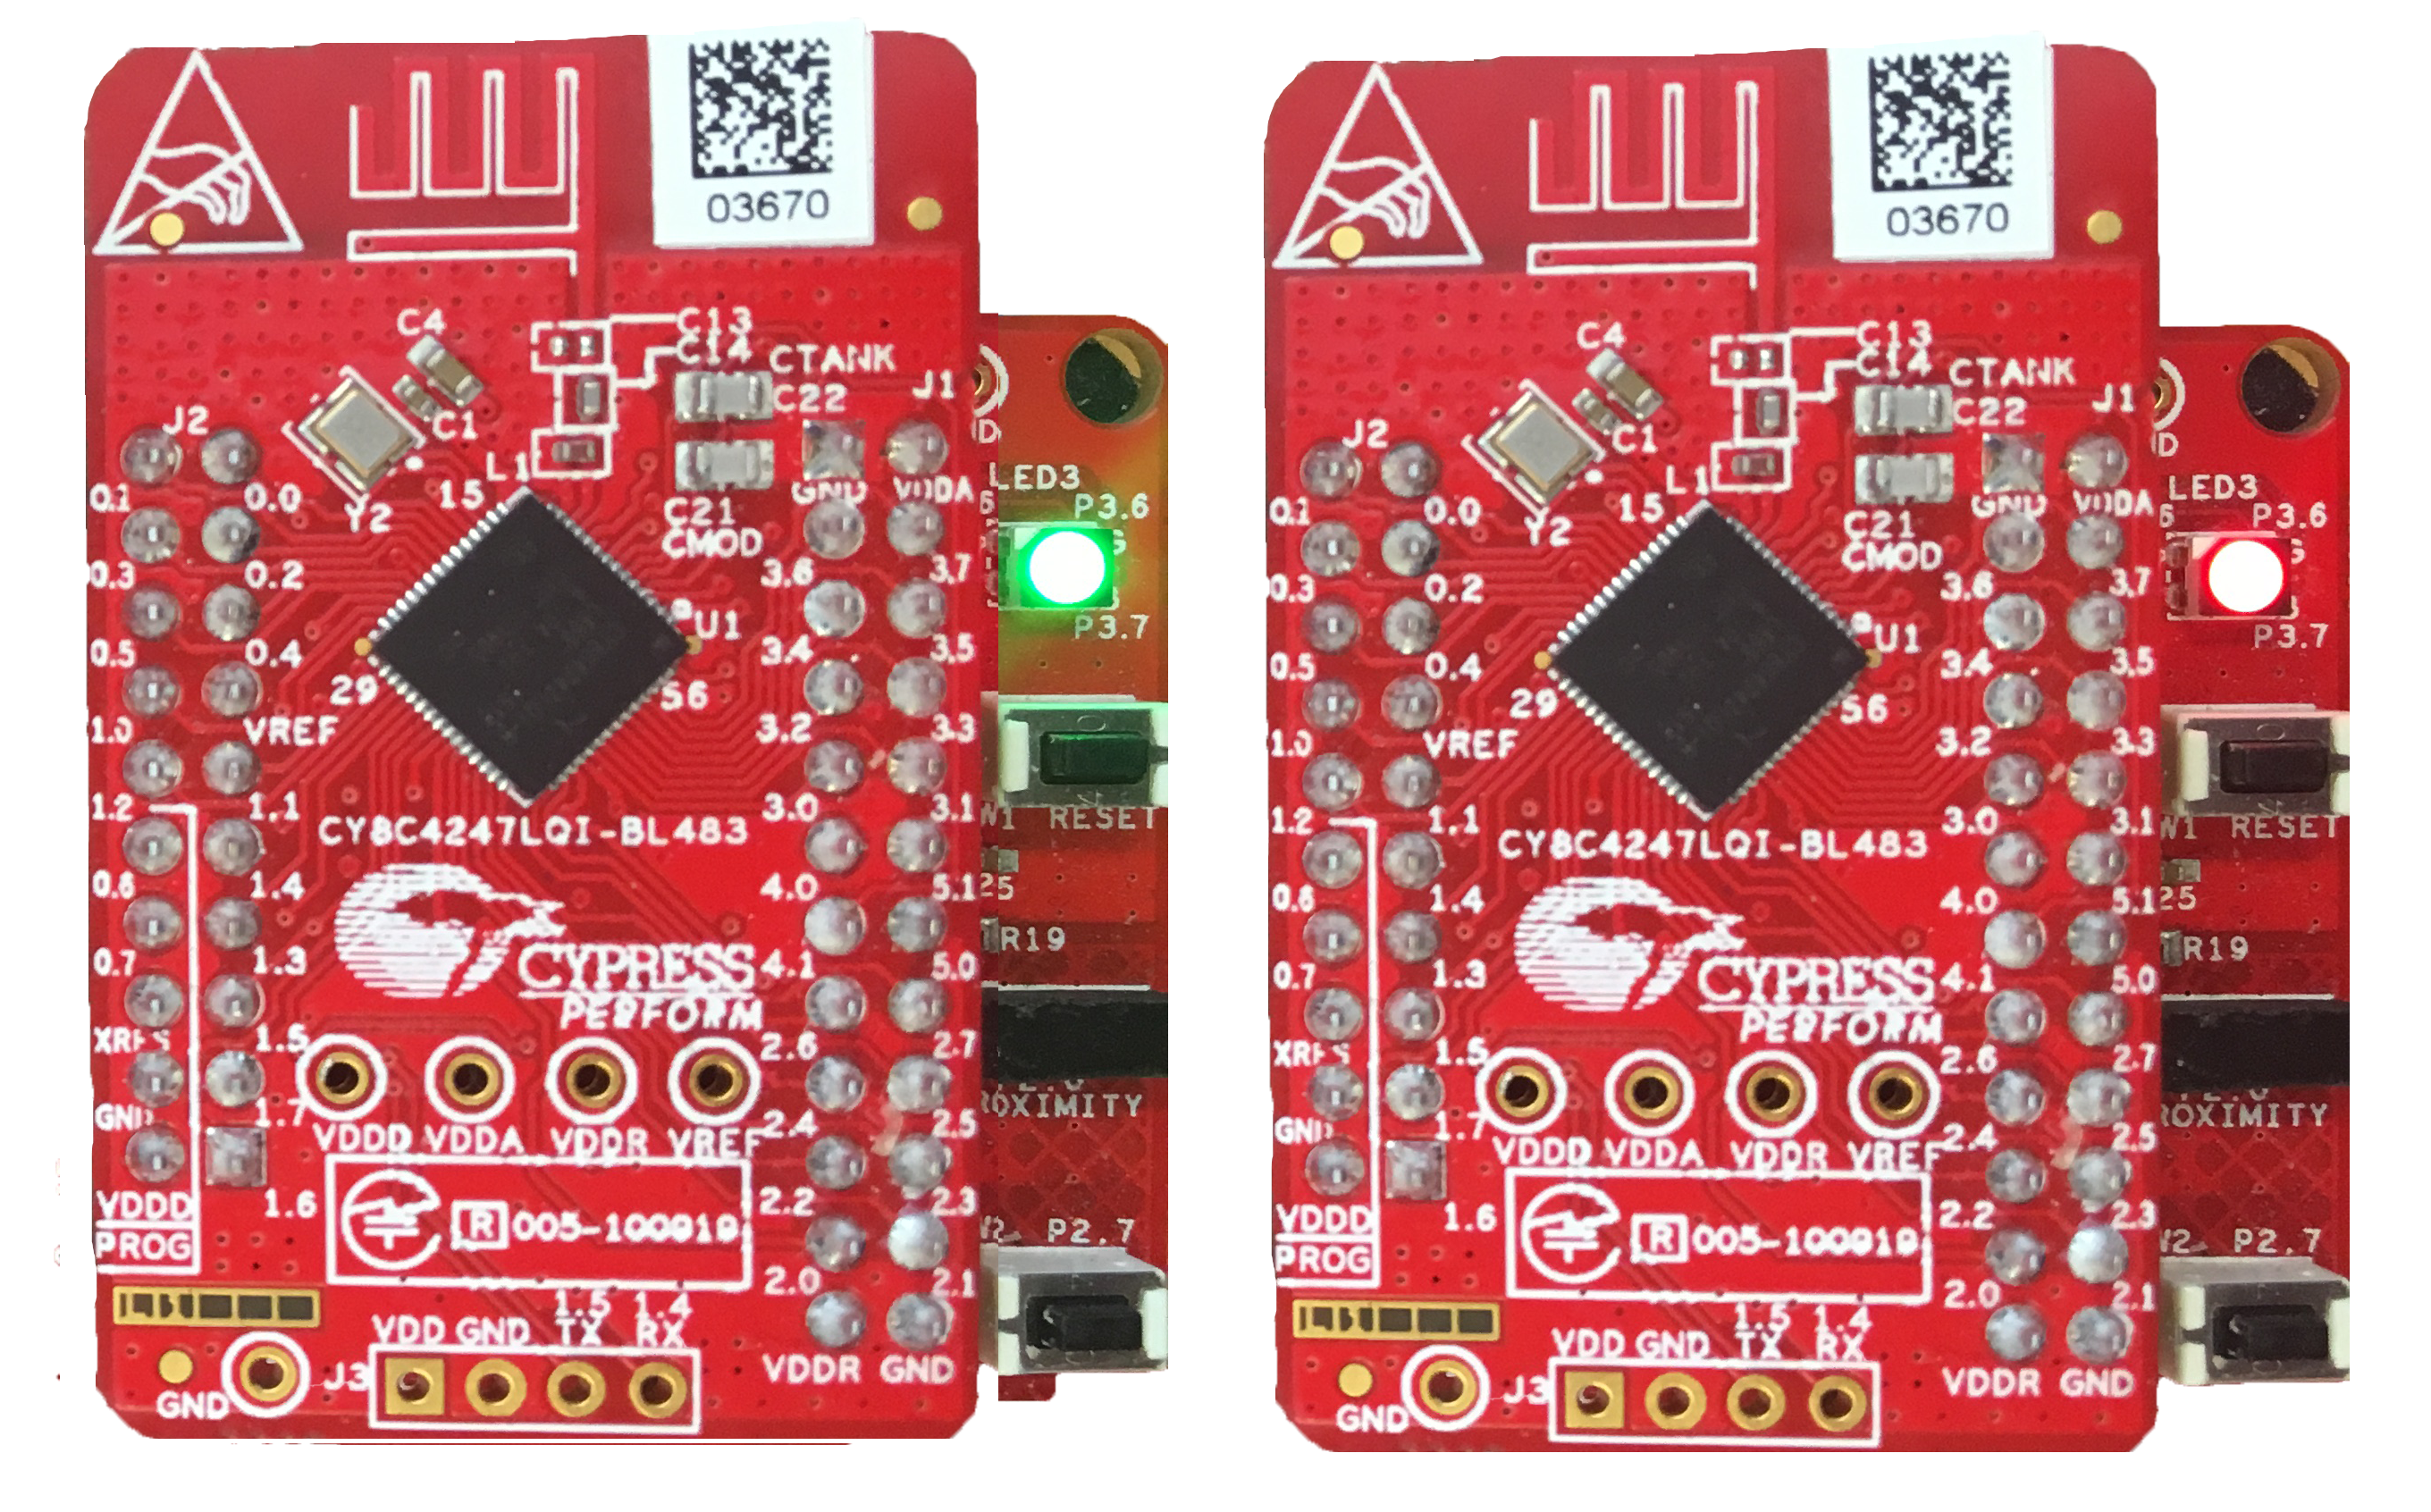
\includegraphics[width=1\textwidth]{figures/mikro_LED}
\caption{Mikrokontrollerens LED ses lyse grøn ved $100^{\circ}$ og lyse rød ved vinkler udenfor $90-180^{\circ}$.}
\label{fig:mikro_LED}
\end{figure}

Ved en overskridelse af grænsen for vinklen, skal det ligeledes visualiseres. Der er foretaget en test, hvorved acceleromterne er påsat en forsøgsperson som overstrækker i knæledder, hvorefter en squat udføres. En visualisering heraf ses af \autoref{fig:vinkeltest_graenser}.

\begin{figure}[H]
\centering
\includegraphics[width=1\textwidth]{figures/vinkeltest_graenser}
\caption{Grafen illustrerer vinklen over knæet under en squat-øvelse. Ved en vinkel under $-100^{\circ}$ symboliseres en overskridelse af grænsen for vinklen. 
\label{fig:vinkeltest_graenser}
\end{figure}

Det ses af \autoref{fig:vinkeltest_graenser}, at forsøgspersonen overstrækker knæleddet, således begge accelerometre overstiger grænsen på $90^{\circ}$, der til sammen udgør en samlet vinkel på $180^{\circ}$. Dette visualiseres ved en vinkel på $-400^{\circ}$. 
Efter 0,5 sekunder ses en vinkel på $-110^{\circ}$, hvilket er gældende, da det ene accelerometer har haft en spænding svarende til præcis $90^{\circ}$ og derfor ikke overskredet grænsen derpå. Ved squat-øvelsen begyndelse ses vinklen falde fra $180-73^{\circ}$, hvorefter den ses stigende igen. Til slut af målingen ses igen et fald under $-100^{\circ}$.



%Disse spændinger kan omregnes til vinkler ved først at finde, hvad spændingen er for én grad ud fra \autoref{tab:vinkelinterval_psoc}  i dét spændingsinterval, hvori den aflæste spænding befinder sig. Det kan aflæses i tabellen, at spændingen fra accelerometeret på femur giver en vinkel mellem 30 og $50^{\circ}$.
%
%\begin{equation}
%\dfrac{-143~V-(-84~V)}{20^{\circ}}=-2,95~V
%\end{equation}
%Derefter findes vinklen for accelerometeret.
%
%\begin{equation}
%\dfrac{-84~V+136~V}{2,95~V}+30^{\circ}=47,627^{\circ}
%\end{equation}
%Ligeledes kan vinklen fra accelerometeret på tibia udregnes til $41,429^{\circ}$. Dette giver en samlet vinkel over leddet: 
%%
%\begin{equation}
%47,627^{\circ}+41,429^{\circ}=89,056^{\circ}
%\end{equation}
%Dette giver en afvigelse på $-1,049~\%$ fra $90^{\circ}$. Denne afvigelse kan godtages til dette systems formål, da der ikke er nogen fare forbundet med, at systemet overskrider de opstillede grænser for vinkler med $-1,049~\%$.

\noindent
En yderligere test er foretaget for at undersøge forsinkelsen af vinkelberegning. Denne test er udført ved at definere en debug-pin, hvor pinen ved funktionskaldet sættes høj og lav efterfølgende. For at illustrere disse målinger tilsluttes et oscilloskop pinen, hvorved der måles hvornår denne er høj. Resultatet af denne test gav en forsinkelse på  $3.6~\mu~s$. Dette betragtes ikke som værende af signifikant betydning, hvorfor denne forsinkelse accepteres.


\vspace{3mm}
\textbf{Opsummering af krav:}
\begin{itemize}
\item[\text{\sffamily \checkmark}] Skal kunne udsende ét signal som repræsenterer en given vinkel
\item[\text{\sffamily \checkmark}] Skal kunne måle knæets vinkel mellem $180^{\circ}$ og $90^{\circ}$
\begin{itemize}
\item En grøn LED skal lyse, når knæets vinkel befinder sig inden for dette interval
\end{itemize}
\item[\text{\sffamily \checkmark}] Skal indikere, hvornår knæets vinkel er over $180^{\circ}$ og under $90^{\circ}$
\begin{itemize}
\item En rød LED skal lyse, hvis knæets vinkel er over $180^{\circ}$ eller under $90^{\circ}$
\end{itemize}
\item[\text{\sffamily \checkmark}] Skal indikere, hvornår knæet overstrækkes, hvilket svarer til $180^{\circ}$
\begin{itemize}
\item Hvis vinklen for ét accelerometer overstiger $90^{\circ}$, indikeres dette som $-200^{\circ}$, hvortil det andet accelerometers vinkel ligges til de $-200^{\circ}$
\item Hvis vinklen overstiger $90^{\circ}$ for hvert accelerometer, skal dette indikeres som et output på $-400^{\circ}$
\end{itemize}
\end{itemize}
%\iffalse
\begingroup
\raggedright

\bibliographystyle{unsrtnat}
\bibliography{kilder}

\endgroup

%-----------------------Bilag-------------------------
\appendix
\chapter{Bilag}
\section{Pilotforsøg} 
\label{sec:pilotforsoeg}
I dette bilag beskrives pilotforsøgets fremgangsmåde samt, hvilke resultater, der opsamles. 

\subsection{Formål}
Dette pilotforsøg har til formål at kunne præcisere samt optimere kravspecifikationerne i de enkelte blokke, hvorved uklare parametre forventes besvaret ud fra pilotforsøgets resultater. Disse parametre omfatter identificering af støjsignaler samt EMG-signalets frekvensområde, da der ses variation i liiteraturen. Parametrene vil forsøges besvaret ud fra målinger ved udførelse af en squat-øvelse.
Hertil anvendes elektroder og to accelerometre som sensorer. På baggrund af dette opstilles følgende formål:  

\subsubsection{EMG-måling}
\begin{enumerate}
\item Opsamling af signal fra rectus femoris % og biceps femoris
	\begin{itemize}
	\item Identificering af frekvensområde
	\item Identificering af støjsignaler 
	\end{itemize}
%\item Identificering af gain til mikroprocesserens operationsspænding \fxnote{Finde operationsspænding og angiv den her}
\end{enumerate}

\subsubsection{Accelerometer-måling}
\begin{enumerate}
\item Identificering af støjsignaler 
\item Identificering af knæleddets vinkel
\end{enumerate}

\subsection{Materialer} 
\begin{itemize}
\item EMG-forstærker, Muscle Sensor V3
\item Elektroder
\item Desinfektionsservietter
\item Skraber
\item To accelerometre ADXL335Z
\item Tape
\item Tusch
\item Breadboards
\item Linial 
\item Vinkelmåler
\item Computer med Scopelogger og MATLAB
\item Ni USB-6009
\item USB-isolater USI-01
\end{itemize}

\subsection{Forsøgsopstilling}
%Til forsøget benyttes to EMG-forstærkere. Dette giver to sæt elektroder til differensmåling af henholdsvis rectus femoris og biceps femoris. Hvert sæt elektroder består af én positiv-, negativ- samt én referenceelektrode. 
%For at identificere elektrodeplacering på musklerne tages der udgangspunkt i Seniam's anvisning for elektrodeplacering \citep{seniam2016}. 
%Elektoderne placeres midt for linjen mellem ischial tuberosity og den laterale epifyse af tibia ved måling over biceps femoris. Ved måling af rectus femoris placeres elektroderne midt for linjen mellem anterior spina iliaca superior og den superior del af patella \citep{seniam2016}. Placeringen af elektroderne illustreres af \autoref{fig:laarmuskler}. 

Til forsøget benyttes en EMG-forstærker, der måler en differensmåling over rectus femoris. Hertil anvendes én positiv-, negativ- samt én referenceelektrode. Forinden påsættelse af elektroder, prepereres huden for således at fjerne hår samt døde hudceller.
For at identificere elektrodeplacering på musklen tages der udgangspunkt i SENIAM's anvisning for elektrodeplacering \citep{seniam2016}. 
Elektoderne placeres midt for linjen mellem anterior spina iliaca superior og den superior del af patella \citep{seniam2016}. Placeringen af elektroderne illustreres af \autoref{fig:laarmuskler}.

\begin{figure}[H]
\centering
\includegraphics[width=0.3\textwidth]{figures/laarmuskel.png}
\caption{Låret set anteriot. Placering af positiv (rød) samt negativ (grøn) elektrode ses på rectus femoris \citep{martini2012}.}
\label{fig:laarmuskler}
\end{figure}

Referenceelektroden placeres, ligeledes efter SENIAM's anvisninger, omkring anklen \citep{seniam2016}. Placeringen af reference elektroden ses af \autoref{fig:reference}.

\begin{figure}[H]
\centering
\includegraphics[width=0.3\textwidth]{figures/reference}
\caption{Placering af referenceelektrode omkring anklen \citep{ankle2016}.}
\label{fig:reference}
\end{figure}

Til forsøget benyttes endvidere to accelerometre, som måler i x, y- samt z-aksen. Disse benyttes for at kunne identificere vinklen af knæet under øvelsen. For så vidt muligt at kunne stabilisere accelerometrene under udførelsen af forsøget, placeres disse på breadboards. 
Som det fremgår af \autoref{fig:accelerometervinkel} placeres det ene accelerometer midt på den laterale side af låret, parallelt med femur. Det andet accelerometer placeres midt på den laterale side af underbenet, parallelt med tibia. Disse breadboards påsættes benet ved brug af tape. Knæets vinkel i oprejst position måler 180$^{\circ}$, hvilket svarer til en 0 g-påvirkning. Vinklen af knæet ændres i takt med udførelse af en squat-øvelse, hvorved g-påvirkningen bevæger sig mod 1. Den samlede vinkel af knæet bestemmes ud fra de to accelerometres parametre. Udregningen for dette kan ses i \autoref{sec:test_acc}.

\begin{figure}[H]
\centering
\includegraphics[width=0.4\textwidth]{figures/accelerometervinkel.png}
\caption{Placering af accelerometrene på låret samt underbenet. Disse placeringer er markeret med rød.}
\label{fig:accelerometervinkel}
\end{figure}

Til identificering af støj fra EMG-forstærkeren fortages der baselinemålinger, som senere analyseres via en frekvensanalyse. Det samme gør sig gældende for identificeringen af EMG-signalets frekvensområde. Dette vil foregå under udførelsen af en squat-øvelse.
En squat-øvelse defineres, således den kan gengives på tværs af forsøgspersonerne.\vspace{3mm}
\begin{enumerate}
\item Forsøgspersonen står i oprejst position. Fødderne placeres med en afstand svarende til ens skulderbredde, hvortil tåspidserne peges let til siderne
\item Armene placeres over kors, som vist på \autoref{fig:squat}
\item Hofte og knæ bøjes således kroppen sænkes kontrolleret. Dette fortsættes indtil en vinkel på 90$^{\circ}$ af knæet er opnået
	\begin{itemize}
	\item Ryggen holdes ret under squat-øvelsen 
	\item Knæene må ikke gå ud over tåspidserne 
	\end{itemize}
\item Kroppen returneres til udgangspunksposition
\end{enumerate} \vspace{3mm}
En illustration af squat-øvelsen ses af \autoref{fig:squat}.

En nedadgående squat-øvelse defineres som punkt $1-2$ i overstående, hertil forbliver forsøgspersonen i en siddende squat indtil den givene måling er gennemført.

For at præcisere øvelsen således alle forsøgspersoner så vidt muligt rammer den samme vinkel på 90$^{\circ}$ af knæet ved gentagende squat-øvelser, måles hver enkel forsøgsperson forinden forsøget udføres. Målingen foregår ved at placere forsøgspersonen på et givent sted med siden til en væg, hvorved en squat-øvelse til 90$^{\circ}$ udføres. De 90$^{\circ}$ måles med en vinkelmåler, hvortil der påsættes tape på væggen, som udgør underbenet samt lårets position.
Ved udførelsen af forsøget irettesætter forsøgspersonen sig efter det påsatte tape på væggen, for således at genskabe squat-øvelsen med mindst mulig afvigelse. Under dette kontrollerer øvrige deltager forsøgspersonens position samt squat-bevægelse.

Da mikrokontrolleren benytter en operationsspænding på $XX~V$ ønskes en signalamplitude under operationsspændingen, da dette vil bidrage til en mindre støjpåvirkning. 
%Noget angående signal to noise ratio 

%For at simulere den påvirkning som accelerometeret udsættes for og derved identificere det maksimale og minimale outputsignal roteres accelerometeret i en langsom rotation fra $0 - 90^{\circ}$ både til højre og venstre. Herudover måles accelerometerets påvirkning i henholdsvis 0 og 1 g-påvirkning for at identificere accelerometeres påvirkning samt, hvorvidt dette stemmer overens med databladet.


\subsection{Oversigt af forsøgsopstilling}
Forsøgsopstillingen ses nedenfor i punktform, for således at give bedre overblik herover. 

\begin{itemize}
\item Identificering af musklen rectus femoris %og biceps femoris 
\item Huden prepereres ved fjernelse af hår og døde hudceller samt desinficering 
\item Elektroderne påsættes
	\begin{itemize}
	\item Positiv og negativ på rectus femoris
	%\item Elektrodesæt 2: positiv og negativ på biceps femoris
	\item Reference på anklen
	\end{itemize} 
\item Accelerometrene placeres 
	\begin{itemize}
	\item Accelerometer 1: midt på den laterale side af låret, parallelt med femur
	\item Accelerometer 2: midt på den laterale side af underbenet, parallelt med tibia 
	\end{itemize}
\item Accelerometrene vælges til at måle i x, y og z-aksen
\end{itemize}

\subsection{Fremgangsmåde}
Forsøgspersonen placeres på et fast punkt under forsøget. Øvelserne udføres tre gange, hvoraf der ud fra målingerne foretages en senere databehandling. 

\subsubsection{Pilotforsøg}
\textbf{Baseline måling}
\begin{itemize}
\item 10 sekunders måling, hvor forsøgspersonen står oprejst
\end{itemize}

\textbf{1. måling}
\begin{itemize}
\item Måling i en nedadgående squat-øvelse
	\begin{itemize}
	\item 1 sekunds baseline oprejst
	\item 4 sekunder nedadgående squat 
	\item 1 sekunds baseline i squat-øvelsen
	\end{itemize}
\end{itemize}
	
\textbf{2. måling}
\begin{itemize}
\item Måling i en squat-øvelse
	\begin{itemize}
	\item 1 sekunds baseline oprejst
	\item 4 sekunder nedadgående squat 
	\item 4 sekunder opadgående squat
	\item 1 sekunds baseline oprejst
	\end{itemize}
\end{itemize}

%\subsubsection{Accelerometer}
%\begin{itemize}
%\item 10 sekunders baseline måling i 0 g-påvirkning (0$^{\circ}$)
%\item 10 sekunders baseline måling i 1 g-påvirkning (90$^{\circ}$)
%\item 10 sekunders måling ved rotation fra $0-1$ g-påvirkning både til højre og venstre
%	\begin{itemize}
%	\item 1 sekunds baseline måling i 0 g-påvirkning (0$^{\circ}$
%	\item 8 sekunders rotation mod 1 g-påvirkning (90$^{\circ}$)
%	\item 1 sekunds baseline måling i 1 g-påvirkning (90$^{\circ}$)
%	\end{itemize}
%\end{itemize}

\section{Databehandling}

\subsection{Accelerometer}
\begin{figure}[H]
\centering
\includegraphics[width=0.5\textwidth]{figures/pilotbase.png}
\caption{Baseline målinger, for forsøgsperson 1 og 2}
\label{fig:navn}
\end{figure}


\begin{figure}[H]
\centering
\includegraphics[width=0.5\textwidth]{figures/pilotmaaling1.png}
\caption{Måling 1, for forsøgsperson 1 og 2}
\label{fig:navn}
\end{figure}


\begin{figure}[H]
\centering
\includegraphics[width=0.5\textwidth]{figures/pilotmaaling2.png}
\caption{Måling 2, for forsøgsperson 1 og 2}
\label{fig:navn}
\end{figure}


\subsection{EMG-måling}


\section{Opsummering af pilotforsøg}
Af resultaterne fra databehandlingen ses det, hvilke parametre, der er nødvendige for optimeret drift af det endelige system. Ud fra frekvensanalysen af EMG-signalerne, ses ingen fremkomst af $50~Hz$ støj.\fxnote{Jeg ved ikke om vi kan antage dette, da frekvensanalysen reelt ikke viser 50 Hz.} Dette antages at skylde envalope kredsen i EMG-forstærkeren. Dette fungerer som et lavpasfilter, hvortil størrelsen af komponenterne i kredsen giver en knækfrekvens på ca. $2~Hz$. Denne udregning fremgår ligeledes af \autoref{eq:lavcutfre}. 
\begin{equation}\label{eq:lavcutfre}
f_c = \frac{1}{2 \pi C R} = \frac{1}{2 \pi*1*10^{-6}F*80,6*10^3\Omega} = 1,94~Hz
\end{equation} 

Af frekvensanalysen fremkommer der dog en dc komponent, som følge af offsette, der ses af EMG-målingerne. \fxnote{ønsker vi at fjerne det offset der fremgår i EMG-målingerne??} Dette giver anledning til, at implementere et højpasfilter, for således at fjerne dc-komponenten. Dette skal dog være med visse forbehold, da frekvensanalysen yderligere viser, at signalet er lavfrekvent. Der ses mest signal fra $0-15~Hz$ ved \autoref{NirushaFrekvensanalyse}. Ved implementering af et højpasfilter, kan det ønskede signal dæmpes i for høj en grad, således signalet ikke vil være anvendeligt. 
 
\subsection{Test af accelerometer} \label{sec:test_acc}
I dette projekt anvendes to accelerometer som sensorer til opsamling af signaler. For at kunne anvende et accelerometer er det vigtigt at kende forskellige tolerancer i forhold til deres datablade, hvorfor et forsøg udføres for at kunne tage højde for disse parametre.

\subsubsection{Formål}
Denne test har til formål at identificere spændingen i henholdsvis $0^{\circ}$ og $90^{\circ}$, hvorudfra vinkler kan beregnes. Derudover identificeres støjsignaler i outputsignalet samt offsettet og sensitiviteten, så dette kan tages højde for i pilotforsøget \autoref{sec:pilotforsøg} og senere forsøg. 

\begin{enumerate}
\item Identificering af spænding ved $0^{\circ}$ og $90^{\circ}$
\item Identificering af støj i outputsignaler for accelerometrene
\item Identificering af offsettet og sensitiviteten for accelerometrene
\end{enumerate}

\subsubsection{Materialer}
\begin{itemize}
\item Accelerometre ADXL$335$
\item Tape
\item Vinkel
\item Vaterpas
\item Breadboard
\item Computer med Scopelogger og MATLAB
\item NI USB-6009
\end{itemize}

\subsubsection{Metode}
Alle målingerne er foretaget i alle tre retninger. 
\begin{enumerate}
\item Der foretages målinger ved $0$ g-påvirkning, hvilket svarer til en hældning på $0^{\circ}$ og ved $1$ g-påvirkning, hvilket svarer til en hældning på $90^{\circ}$
\item Støjsignaler i outputtet identificeres ved måling af baseline uden nogen g-påvirkningen, hvorefter det måles ved $1$ g-påvirkningen. 
\item På baggrund af de forrige mål kan offsettet og sensitiviteten udregnes
\end{enumerate}

\subsubsection{Forsøgsopstilling}
Forsøgsopstillingen udføres på samme måde for begge accelerometre.
\begin{itemize}
\item Accelerometeret tilkobles breadboard og sættes fast med tape.
\item Accelerometeret indstilles så det er vinkelret
\begin{itemize}
\item Accelerometeret placeres efter fremgangsmåden \autoref{acc_fremgangsmaade}
\end{itemize}
\item Accelerometeret tilkobles NI USB-6009
\item NI USB-6009 tilkobles computer
\end{itemize}

\subsubsection{Fremgangsmåde} \label{acc_fremgangsmaade}
Der foretages 6 forskellige målinger for hvert accelerometer. Fremgangsmåden er illustreret på \autoref{fig:acc1} og \autoref{fig:acc2}
\begin{itemize}
\item Accelerometeret er plan på bordet opad
\item Accelerometeret er plan på bordet nedad
\item Accelerometeret er lodret opad
\item Accelerometeret er lodret nedad
\item Accelerometeret er vandret mod højre
\item Accelerometeret er vandret mod venstre
\end{itemize}

\begin{figure}
\centering
\begin{subfigure}{.5\textwidth}
  \centering
  \includegraphics[width=.4\linewidth]{acc1}
  \caption{A subfigure}
  \label{fig:acc1}
\end{subfigure}%
\begin{subfigure}{.5\textwidth}
  \centering
  \includegraphics[width=.4\linewidth]{acc2}
  \caption{A subfigure}
  \label{fig:acc2}
\end{subfigure}
\caption{A figure with two subfigures}
\label{fig:test}
\end{figure}



\subsection{Behandling af data}


%\fi
\end{document}
